\documentclass[11pt,spanish,Letterpaper,openany]{book}
\usepackage{lmodern}
\usepackage{setspace}
\setstretch{1.0}
\usepackage{amssymb,amsmath}
\usepackage{ifxetex,ifluatex}
\usepackage{fixltx2e} % provides \textsubscript
\ifnum 0\ifxetex 1\fi\ifluatex 1\fi=0 % if pdftex
  \usepackage[T1]{fontenc}
  \usepackage[utf8]{inputenc}
\else % if luatex or xelatex
  \ifxetex
    \usepackage{mathspec}
  \else
    \usepackage{fontspec}
  \fi
  \defaultfontfeatures{Ligatures=TeX,Scale=MatchLowercase}
    \setmainfont[]{Corbel}
\fi

\makeatletter
\renewcommand\mainmatter{\clearpage\@mainmattertrue\pagenumbering{arabic}}
\renewcommand\frontmatter{\clearpage\@mainmatterfalse\pagenumbering{roman}}
\renewcommand\backmatter{\clearpage\@mainmatterfalse}
\makeatother

%\usepackage{etoolbox}
%\makeatletter
%\patchcmd{\@smemmain}{\cleardoublepage}{\clearpage}{}{}
%\patchcmd{\@smemmain}{\cleardoublepage}{\clearpage}{}{}
%\patchcmd{\@smemfront}{\cleardoublepage}{\clearpage}{}{}
%\patchcmd{\@smemfront}{\cleardoublepage}{\clearpage}{}{}
%\makeatother

\setlength{\parindent}{0em}

\usepackage{graphicx}
\usepackage{booktabs}
\usepackage{multicol}
\usepackage{doc}
\usepackage{float}
\usepackage{tcolorbox} 
\usepackage{lipsum}
\usepackage{tikz}
\usepackage{nonfloat}

\usepackage{pdfpages}

\usepackage[
contents={},
opacity=1,
scale=1.5,
color=blue!90
]{background}
\usepackage{lipsum}
\usepackage{ifthen}

\usepackage{xcolor}
\usepackage[pagestyles]{titlesec}

\renewpagestyle{plain}[\normalsize\sffamily\bfseries\slshape]{
  \setfoot{}{\color{white}{\thepage}}{}}

\newpagestyle{myps}[\normalsize\sffamily\bfseries\slshape]{
  \setfoot{}{\color{white}{\thepage}}{}}
  
\pagestyle{myps}


\usepackage{framed}
\definecolor{fondo}{HTML}{DCEEA7}%
\colorlet{shadecolor}{fondo!81!}


% use upquote if available, for straight quotes in verbatim environments
\IfFileExists{upquote.sty}{\usepackage{upquote}}{}
% use microtype if available
\IfFileExists{microtype.sty}{%
\usepackage{microtype}
\UseMicrotypeSet[protrusion]{basicmath} % disable protrusion for tt fonts
}{}
\usepackage[inner=30mm,outer=20mm,top=25mm,bottom=21.0mm]{geometry}
\usepackage{hyperref}
\hypersetup{unicode=true,
            pdftitle={Revista de la Unidad de Prácticas de Ingeniería y EPS},
            pdfauthor={Unidad de Prácticas de Ingeniería y EPS},
            pdfborder={0 0 0},
            breaklinks=true}
\urlstyle{same}  % don't use monospace font for urls
\ifnum 0\ifxetex 1\fi\ifluatex 1\fi=0 % if pdftex
  \usepackage[shorthands=off,main=spanish]{babel}
\else
  \usepackage{polyglossia}
  \setmainlanguage[]{spanish}
\fi
\usepackage{natbib}
\bibliographystyle{apalike}
\usepackage{longtable,booktabs}
\usepackage{graphicx,grffile}
\makeatletter
\def\maxwidth{\ifdim\Gin@nat@width>\linewidth\linewidth\else\Gin@nat@width\fi}
\def\maxheight{\ifdim\Gin@nat@height>\textheight\textheight\else\Gin@nat@height\fi}
\makeatother
% Scale images if necessary, so that they will not overflow the page
% margins by default, and it is still possible to overwrite the defaults
% using explicit options in \includegraphics[width, height, ...]{}
\setkeys{Gin}{width=\maxwidth,height=\maxheight,keepaspectratio}
\IfFileExists{parskip.sty}{%
\usepackage{parskip}
}{% else
\setlength{\parindent}{0pt}
\setlength{\parskip}{6pt plus 2pt minus 1pt}
}
\setlength{\emergencystretch}{3em}  % prevent overfull lines
\providecommand{\tightlist}{%
  \setlength{\itemsep}{0pt}\setlength{\parskip}{0pt}}
\setcounter{secnumdepth}{5}
% Redefines (sub)paragraphs to behave more like sections
\ifx\paragraph\undefined\else
\let\oldparagraph\paragraph
\renewcommand{\paragraph}[1]{\oldparagraph{#1}\mbox{}}
\fi
\ifx\subparagraph\undefined\else
\let\oldsubparagraph\subparagraph
\renewcommand{\subparagraph}[1]{\oldsubparagraph{#1}\mbox{}}
\fi

%%% Use protect on footnotes to avoid problems with footnotes in titles
\let\rmarkdownfootnote\footnote%
\def\footnote{\protect\rmarkdownfootnote}


  \title{Revista de la Unidad de Prácticas de Ingeniería y EPS}
    \author{Unidad de Prácticas de Ingeniería y EPS}
      \date{2019-07-22}

% no title page
\AtBeginDocument{\let\maketitle\relax}

\usepackage{booktabs}
\usepackage{longtable}

\usepackage{indentfirst}
\setlength{\parindent}{1em}
\usepackage{enumitem}
\setlist[itemize]{labelindent = \parindent, leftmargin=*}

%\usepackage{framed,color}
%\definecolor{shadecolor}{RGB}{248,248,248}

\renewcommand{\textfraction}{0.05}
\renewcommand{\topfraction}{0.8}
\renewcommand{\bottomfraction}{0.8}
\renewcommand{\floatpagefraction}{0.75}

\renewcommand{\chaptername}{Artículo}
\addto\captionsspanish{\renewcommand{\chaptername}{Artículo}}

\frenchspacing
\tolerance=5000
\multicoltolerance=3000 

\raggedbottom
\raggedcolumns

\setlength{\columnsep}{1.5em}
%We want a rule between columns.
%\setlength\columnseprule{.4pt}

%Tambien queremos asegurarnos de que un nuevo entorno multicols 
%encuentre suficiente espacio en la parte inferior de la pagina.
\setlength\premulticols{6\baselineskip}

%Al equilibrar columnas, ignoramos las soluciones que son 
%demasiado malas. Ademas, si la ultima columna es demasiado mala, 
%la tipeamos sin estirar.
\setcounter{columnbadness}{7000}
\setcounter{finalcolumnbadness}{7000}


\newcommand{\photocommand}[2]{%
\fcolorbox[HTML]{DCEEA7}{DCEEA7}{%
\begin{minipage}{95.19mm}%
	\hspace{1mm}%
	\begin{minipage}{22.49mm}%
		\vspace{1mm}%
		\includegraphics[width=22.49mm, height=31.96mm]{#1}%
		\vspace{1mm}%
	\end{minipage}%
	\hspace{2.4mm}%
	\begin{minipage}{68.80mm}%
		#2
	\end{minipage}%
	\hspace{0.5mm}%
\end{minipage}%
}%
}

\definecolor{fondobiography}{HTML}{DCEEA7}

\NewDocumentEnvironment{photobiography}{m O{}}%
{%
\begin{tcolorbox}[colback=fondobiography, colframe=fondobiography, width=97.19mm, boxsep=-2mm, arc=0mm]
\begin{minipage}{95.19mm}%
	%\hspace{1mm}%
	\begin{minipage}{22.49mm}%
		\vspace{2mm}%
		\includegraphics[width=22.49mm, height=31.96mm]{#1}%
		\vspace{2mm}%
	\end{minipage}%
	\hspace{2.4mm}%
	\begin{minipage}{68.80mm}%
	#2%
}%
{%
	\end{minipage}%
	%\hspace{0.5mm}%
\end{minipage}%
\end{tcolorbox}
}

\begin{document}
\maketitle

% \pagestyle{plain}
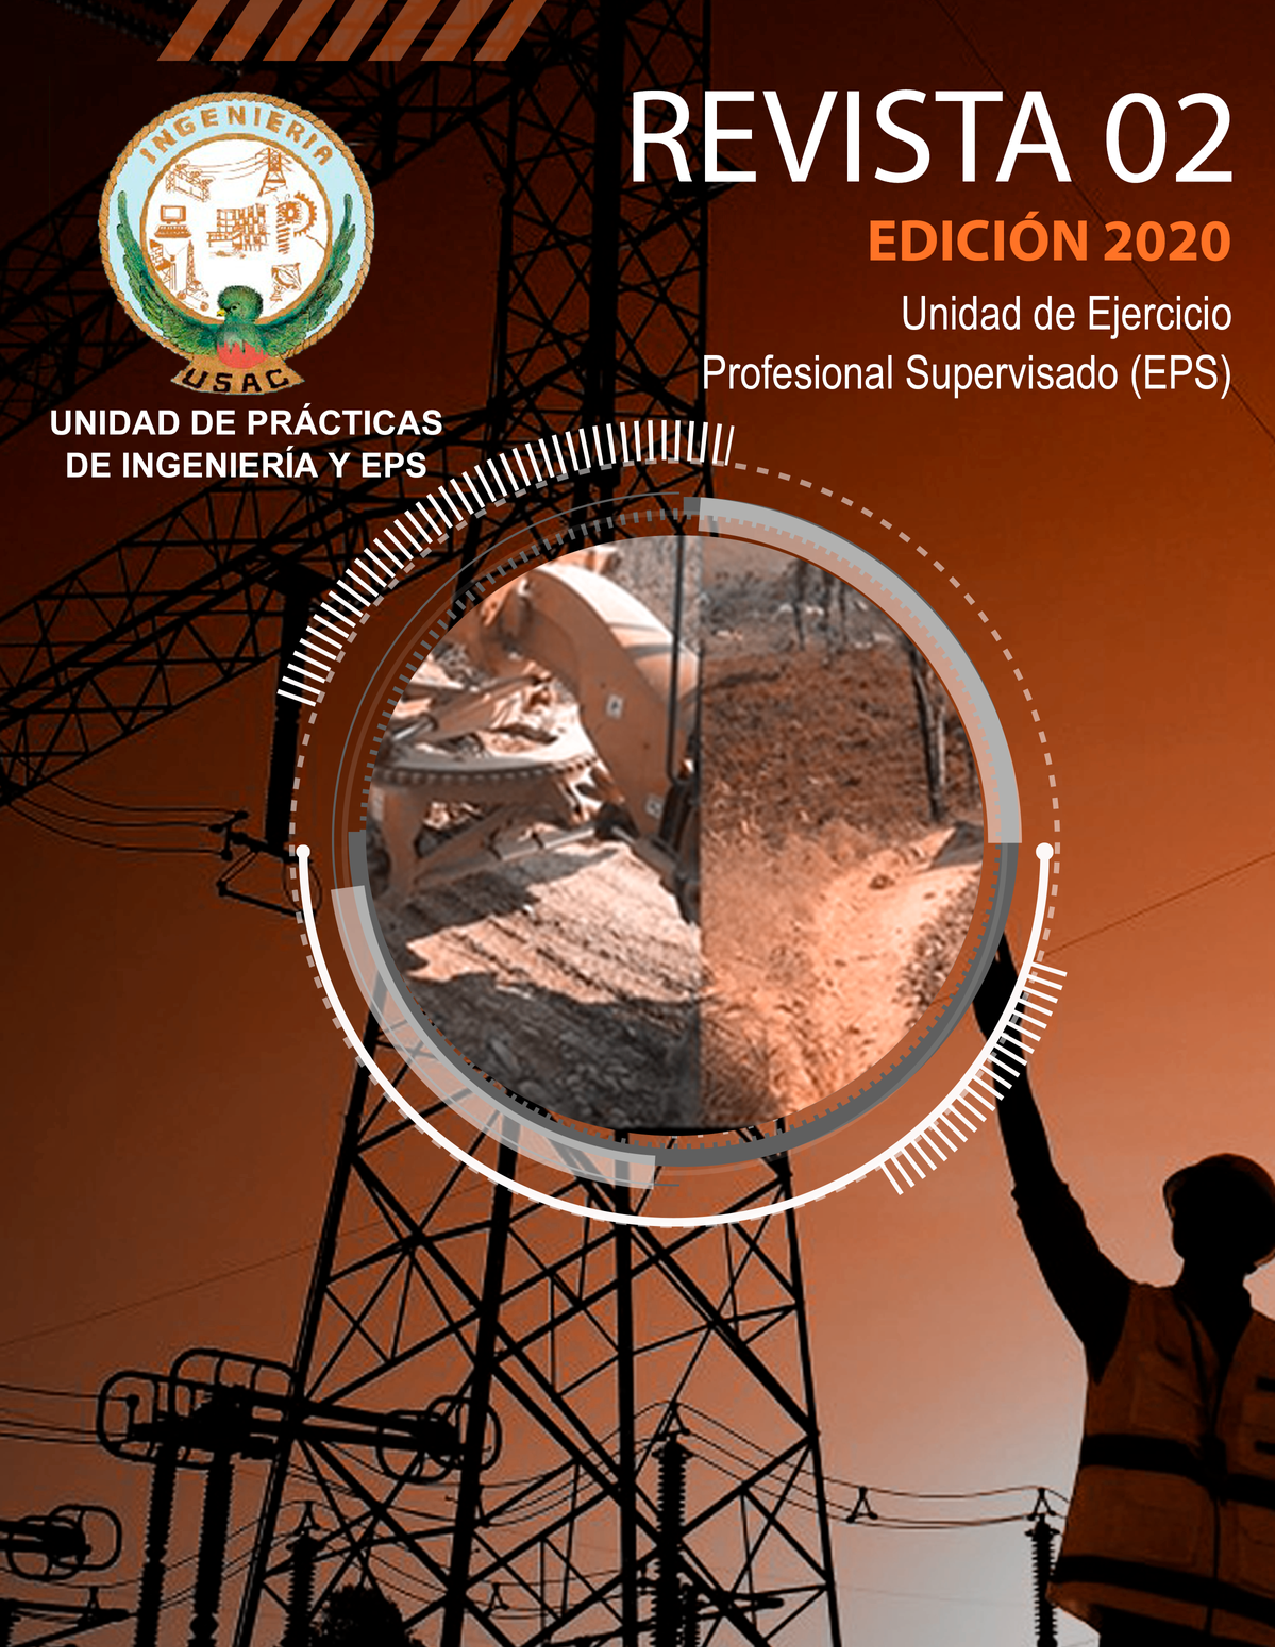
\includepdf{images/cover.pdf}

\AddEverypageHook{%
\ifnum  \value{page}<34%
  \ifthenelse{\isodd{\value{page}}}%
  	{\backgroundsetup{scale=1, color=black, opacity=1, angle=0, contents={
\includegraphics[width=\paperwidth,height=\paperheight]{images/background_numberimpar.png}}}}%
  	{\backgroundsetup{scale=1, color=black, opacity=1, angle=0, contents={
\includegraphics[width=\paperwidth,height=\paperheight]{images/background_numberpar.png}}}}%
\fi%
\BgMaterial}

%%%%%%{
%%%%%%\setcounter{tocdepth}{0}
%%%\tableofcontents
%%%}
%%%%%%%%%%%%\listoffigures
%%%
\frontmatter

\titleformat{\chapter}[display]{\bfseries\Large}{\relax}{0ex}{\titlerule\filright}[\vspace{1ex}\titlerule]

\titlespacing*{\chapter} {0pt}{50pt}{40pt}

\hypertarget{index}{%
\chapter*{Editorial}\label{index}}
\addcontentsline{toc}{chapter}{Editorial}

Dentro de las políticas de la Universidad de San Carlos de Guatemala está la extensión de sus diferentes unidades; en el caso de la Facultad de Ingeniería, es por medio de la Unidad de EPS donde se retribuye el aporte de la población guatemalteca a la USAC a través de los impuestos, con la elaboración de proyectos de beneficio comunitario; además, es importante la participación del futuro profesional en el área laboral de empresas privadas y de instituciones públicas, potque son los espacios en los cuales se desenvuelve un alto porcentaje de egresados de la Facultad. Algunas veces no se da a conocer la importancia de la divulgación y alcance de la participación de los futuros profesionales, así como de la Facultad de Ingeniería de la Universidad de San Carlos de Guatemala; por ello, es importante resaltar y transmitir el aporte en la práctica de sus futuros graduandos.

Para el desarrollo integral de nuestro país, Guatemala, es indispensable que las carreras técnicas como la ingeniería, en sus diversas ramas, se desarrollen con tecnologías modernas y estrategias educativas actualizadas. El principal objetivo de la Unidad de Prácticas de Ingeniería y EPS es relacionar la teoría con la práctica; como un complemento para consolidar dicho fin surge la presente revista denominada ``Unidad de Prácticas de Ingeniería y EPS'', cuyo contenido tiene como fin motivar al estudiante para que realice proyectos que signifiquen soluciones a problemas reales planteados en cada comunidad o empresa. Por lo tanto, el aporte de los estudiantes de ingeniería con la asesoría de los profesionales de la Unidad de EPS, se centra en la aplicabilidad de los conocimientos adquiridos en aras del beneficio de la población guatemalteca.

La presente revista constituirá el espacio cultural y científico para que los catedráticos y estudiantes de la Facultad de Ingeniería publiquen sus experiencias a través de interesantes artículos, cuyo contenido permita generar y consolidar el conocimiento de la ingeniería, y motive, por ende, al estudiante para ser un profesional exitoso en el campo de su especialidad.

Esta revista será el espacio de apertura a la discusión y generación de conocimientos aportados a través de la creatividad e innovación, con las ideas de estudiantes y catedráticos; de esa manera podrá cimentarse un mundo diverso de posibilidades que permita informar apropiadamente todo lo que concierne a la práctica supervisada y al conocimiento científico adquirido; esto propiciará el desarrollo académico y profesional, tanto de la Facultad de Ingeniería como de la Universidad de San Carlos de Guatemala.
\bigskip
\bigskip
\bigskip

\begin {center}

\textbf{Ing. Oscar Argueta Hernández}\\
Director de la Unidad de EPS USAC

\end {center}

\newpage

\hypertarget{directorio}{%
\chapter*{Directorio}\label{directorio}}
\addcontentsline{toc}{chapter}{Directorio}

\hypertarget{director-de-la-revista}{%
\subsection*{Director de la Revista}\label{director-de-la-revista}}
\addcontentsline{toc}{subsection}{Director de la Revista}

\textbf{Ingeniero Oscar Argueta Hernández}\\
Dirección de Prácticas de Ingeniería y EPS
\bigskip

\hypertarget{editor-en-jefe}{%
\subsection*{Editor en Jefe}\label{editor-en-jefe}}
\addcontentsline{toc}{subsection}{Editor en Jefe}

\textbf{Ingeniera Floriza Avila Pesquera de Medinilla}\\
Coordinadora del Área de Tecnología\\
Unidad de Prácticas de Ingeniería
\bigskip

\hypertarget{coeditores}{%
\subsection*{Coeditores}\label{coeditores}}
\addcontentsline{toc}{subsection}{Coeditores}

\textbf{Ingeniero Juan Merck Cos}\\
Asesor Supervisor del Área de Ingeniería Civil\\
Unidad de Prácticas de Ingeniería
\bigskip

\textbf{Ingeniero Silvio José Rodríguez Serrano}\\
Asesor Supervisor del Área de Ingeniería Civil\\
Unidad de Prácticas de Ingeniería
\bigskip

\textbf{Ingeniera Sigrid Alitza Calderón de De Léon}\\
Asesor Supervisor del Área de Ingeniería Industrial y Mécanica Industrial\\
Unidad de Prácticas de Ingeniería

\hypertarget{consejo-editorial}{%
\section*{Consejo Editorial}\label{consejo-editorial}}
\addcontentsline{toc}{section}{Consejo Editorial}

\textbf{Ingeniero Oscar Argueta Hernández}\\
Asesor Supervisor del Área de Ingeniería Civil\\
Unidad de Prácticas de Ingeniería
\bigskip

\textbf{Ingeniera Floriza Avila Pesquera de Medinilla}\\
Asesor Supervisor del Área de Ingeniería de Ciencias y Sistemas\\
Unidad de Prácticas de Ingeniería
\bigskip

\textbf{Ingeniero Juan Merck Cos}\\
Asesor Supervisor del Área de Ingeniería Civil\\
Unidad de Prácticas de Ingeniería
\bigskip

\textbf{Ingeniero Carlos Anibal Chicojay Coloma}\\
Asesor Supervisor del Área de Ingeniería Mécanica\\
Unidad de Prácticas de Ingeniería
\bigskip

\textbf{Ingeniera Sigrid Alitza Calderón de De Léon}\\
Asesor Supervisor del Área de Ingeniería Industrial y Mécanica Industrial\\
Unidad de Prácticas de Ingeniería
\bigskip

\textbf{Ingeniera Norma Ileana Sarmiento de Serrano}\\
Asesor Supervisor del Área de Ingeniería Industrial y Mécanica Industrial\\
Unidad de Prácticas de Ingeniería

\hypertarget{comite-editorial}{%
\section*{Comité Editorial}\label{comite-editorial}}
\addcontentsline{toc}{section}{Comité Editorial}

\textbf{Ingeniero Oscar Argueta Hernández}\\
Asesor Supervisor del Área de Ingeniería Civil\\
Unidad de Prácticas de Ingeniería
\bigskip

\textbf{Ingeniera Floriza Avila Pesquera de Medinilla}\\
Asesor Supervisor del Área de Ingeniería de Ciencias y Sistemas\\
Unidad de Prácticas de Ingeniería
\bigskip

\textbf{Ingeniero Juan Merck Cos}\\
Asesor Supervisor del Área de Ingeniería Civil\\
Unidad de Prácticas de Ingeniería
\bigskip

\textbf{Ingeniero Carlos Anibal Chicojay Coloma}\\
Asesor Supervisor del Área de Ingeniería Mécanica\\
Unidad de Prácticas de Ingeniería
\bigskip

\textbf{Ingeniera Sigrid Alitza Calderón de De Léon}\\
Asesor Supervisor del Área de Ingeniería Industrial y Mécanica Industrial\\
Unidad de Prácticas de Ingeniería
\bigskip

\textbf{Ingeniera Norma Ileana Sarmiento de Serrano}\\
Asesor Supervisor del Área de Ingeniería Industrial y Mécanica Industrial\\
Unidad de Prácticas de Ingeniería
\bigskip

\textbf{Ingeniero Silvio José Rodríguez Serrano}\\
Asesor Supervisor del Área de Ingeniería Civil\\
Unidad de Prácticas de Ingeniería
\bigskip

\setcounter{tocdepth}{0}
\tableofcontents

\mainmatter

\titleformat{\chapter}[display]{\bfseries\Large}{\filleft\MakeUppercase{\string Artículo}}{55pt}{\titlerule\filright}[\vspace{1ex}\titlerule]

\titlespacing*{\chapter} {0pt}{-55pt}{20pt}

\hypertarget{unidadeps}{%
\chapter[Unidad de Prácticas de Ingeniería y Ejercicio Profesional Supervisado ]{\texorpdfstring{Unidad de Prácticas de Ingeniería y Ejercicio Profesional Supervisado \footnote{\url{http://eps.ingenieria.usac.edu.gt/}}}{Unidad de Prácticas de Ingeniería y Ejercicio Profesional Supervisado }}\label{unidadeps}}

\begin {flushleft}

\begin{tcolorbox}[sharp corners=uphill, colback=fondo, colframe=fondo, arc=6mm, boxrule=0mm, boxsep=2mm,  opacityframe=0.19,  opacityback=0.19]

\begin{minipage}[c]{3cm}


\includegraphics[width=2.5cm,height=\textheight]{images/201901-usac-logo.jpg}

\end{minipage}\begin{minipage}[c]{12cm}

\emph{La Unidad de Ejercicio Profesional Supervisado (EPS) es la Unidad oficial encargada de administrar y darle seguimiento a los programas de Ejercicio Profesional Supervisado de Graduación de la Facultad de Ingeniería, en coordinación con las diferentes escuelas.}

\end{minipage}

\end {tcolorbox}

\end {flushleft}
\smallskip

\begin {multicols}{2}

\hypertarget{introduccion}{%
\section*{Introducción}\label{introduccion}}
\addcontentsline{toc}{section}{Introducción}

La Unidad de Ejercicio Profesional Supervisado (EPS) depende directamente de la Decanatura de la Facultad de Ingeniería, es la Unidad oficial encargada de administrar y darle seguimiento a los programas de Ejercicio Profesional Supervisado de Graduación de la Facultad de Ingeniería, en coordinación con las diferentes escuelas.

La Universidad de San Carlos de Guatemala, a través de sus diferentes programas de extensión, permite una vinculación con la sociedad guatemalteca, contribuyendo a la solución de la problemática nacional y al mejoramiento de la calidad de vida de sus habitantes.

Dentro de estos programas, la Facultad de Ingeniería cuenta con el Ejercicio Profesional Supervisado (E.P.S.), trabajando en coordinación con diferentes instituciones públicas y privadas como: Municipalidades, Ministerios, Cooperativas, Organismos No Gubernamentales, Ingenios Azucareros, Fundaciones, Hospitales, Dependencias de la Universidad de San Carlos de Guatemala, etc.

El EPS incluye actividades académicas de servicio técnico-profesional universitario de investigación y docencia-aprendizaje que los estudiantes con cierre de pénsum de estudios realizan en el medio real del país, para resolver problemas relativos a su profesión.

Por medio de esta práctica, los estudiantes próximos a graduarse, ejercitan su profesión, apoyados y orientados por los asesores-supervisores docentes, para formar profesionalmente a los estudiantes y prestar servicios a la sociedad.

\hypertarget{mision}{%
\section*{Misión}\label{mision}}
\addcontentsline{toc}{section}{Misión}

Complementar y fortalecer la formación académica de los estudiantes de las distintas carreras de la Facultad de Ingeniería de la Universidad de San Carlos de Guatemala, a través de la realización de las Prácticas de Ingeniería y el Ejercicio Profesional Supervisado, aplicando los conocimientos, habilidades (destrezas) y criterios adquiridos durante la formación académica a problemas reales a los que se enfrentará, adquiriendo conciencia de la realidad nacional, formándose como un futuro profesional comprometido con el desarrollo del país, en su entorno social y ecológico.

\hypertarget{vision}{%
\section*{Visión}\label{vision}}
\addcontentsline{toc}{section}{Visión}

Ser la dependencia de la Facultad de Ingeniería que complemente la formación profesional de los estudiantes de las diferentes especialidades de la Ingeniería, para que integren los conocimientos, habilidades (destrezas) y criterios adquiridos durante su carrera, con el fin de formar profesionales con principios éticos y excelencia académica comprometidos a integrarse en los diversos sectores de la sociedad.

\hypertarget{objetivos}{%
\section*{Objetivos}\label{objetivos}}
\addcontentsline{toc}{section}{Objetivos}

\hypertarget{general}{%
\subsection*{General}\label{general}}
\addcontentsline{toc}{subsection}{General}

Sistematizar y enriquecer los conocimientos del estudiante al interpretar objetivamente la realidad nacional, mediante la confrontación cotidiana de la teoría con la práctica.

\hypertarget{especificos}{%
\subsection*{Específicos}\label{especificos}}
\addcontentsline{toc}{subsection}{Específicos}

\begin{itemize}
\item
  Participar en las diferentes comunidades, instituciones y empresas asignadas como centros de Prácticas a través del Ejercicio Profesional Supervisado de la Facultad de Ingeniería de la Universidad de San Carlos de Guatemala; dándole prioridad a aquellas que realicen actividades no lucrativas o que realicen funciones de interés social.
\item
  Generar un proceso de participación y auto-gestión en las comunidades, instituciones y empresas, a fin de promover o fortalecer su organización como instrumento para el impulso del desarrollo social permanentemente y sostenible.
\item
  Fortalecer la formación profesional de los futuros egresados, mediante un trabajo supervisado que integre y aplique los conocimientos adquiridos durante la carrera.
\item
  Contribuir a que los estudiantes desarrollen la capacidad de análisis e interpretación de la problemática nacional.
\item
  Promover las actividades de docencia, investigación y extensión universitaria con participación inter-institucional en el ámbito nacional.
\end{itemize}

\hypertarget{organigrama}{%
\section*{Organigrama}\label{organigrama}}
\addcontentsline{toc}{section}{Organigrama}

La Unidad de EPS, cuenta con una estructura organizacional jerárquica, en donde el primer nivel lo constituye el Director de la Unidad de EPS, en el segundo nivel los Coordinadores de cada área y en el tercer nivel se encuentran los Asesores-Supervisores.
\bigskip

\begin {flushleft}

\noindent\begin{minipage}[c]{\columnwidth}

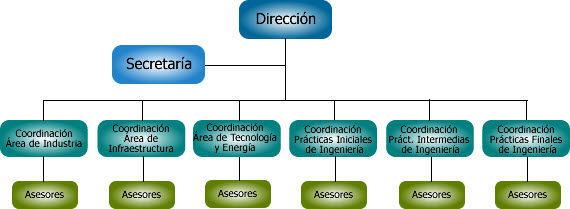
\includegraphics[width=1\linewidth]{images/201901-unidadeps-imagen01}
\figcaption{Organigrama Unidad de Prácticas de Ingeniería y EPS}

\end{minipage}

\end {flushleft}

\bigskip

\end {multicols}

\hypertarget{personal-administrativo-y-docente}{%
\section*{Personal Administrativo y Docente}\label{personal-administrativo-y-docente}}
\addcontentsline{toc}{section}{Personal Administrativo y Docente}

\begin{figure}[H]

{\centering 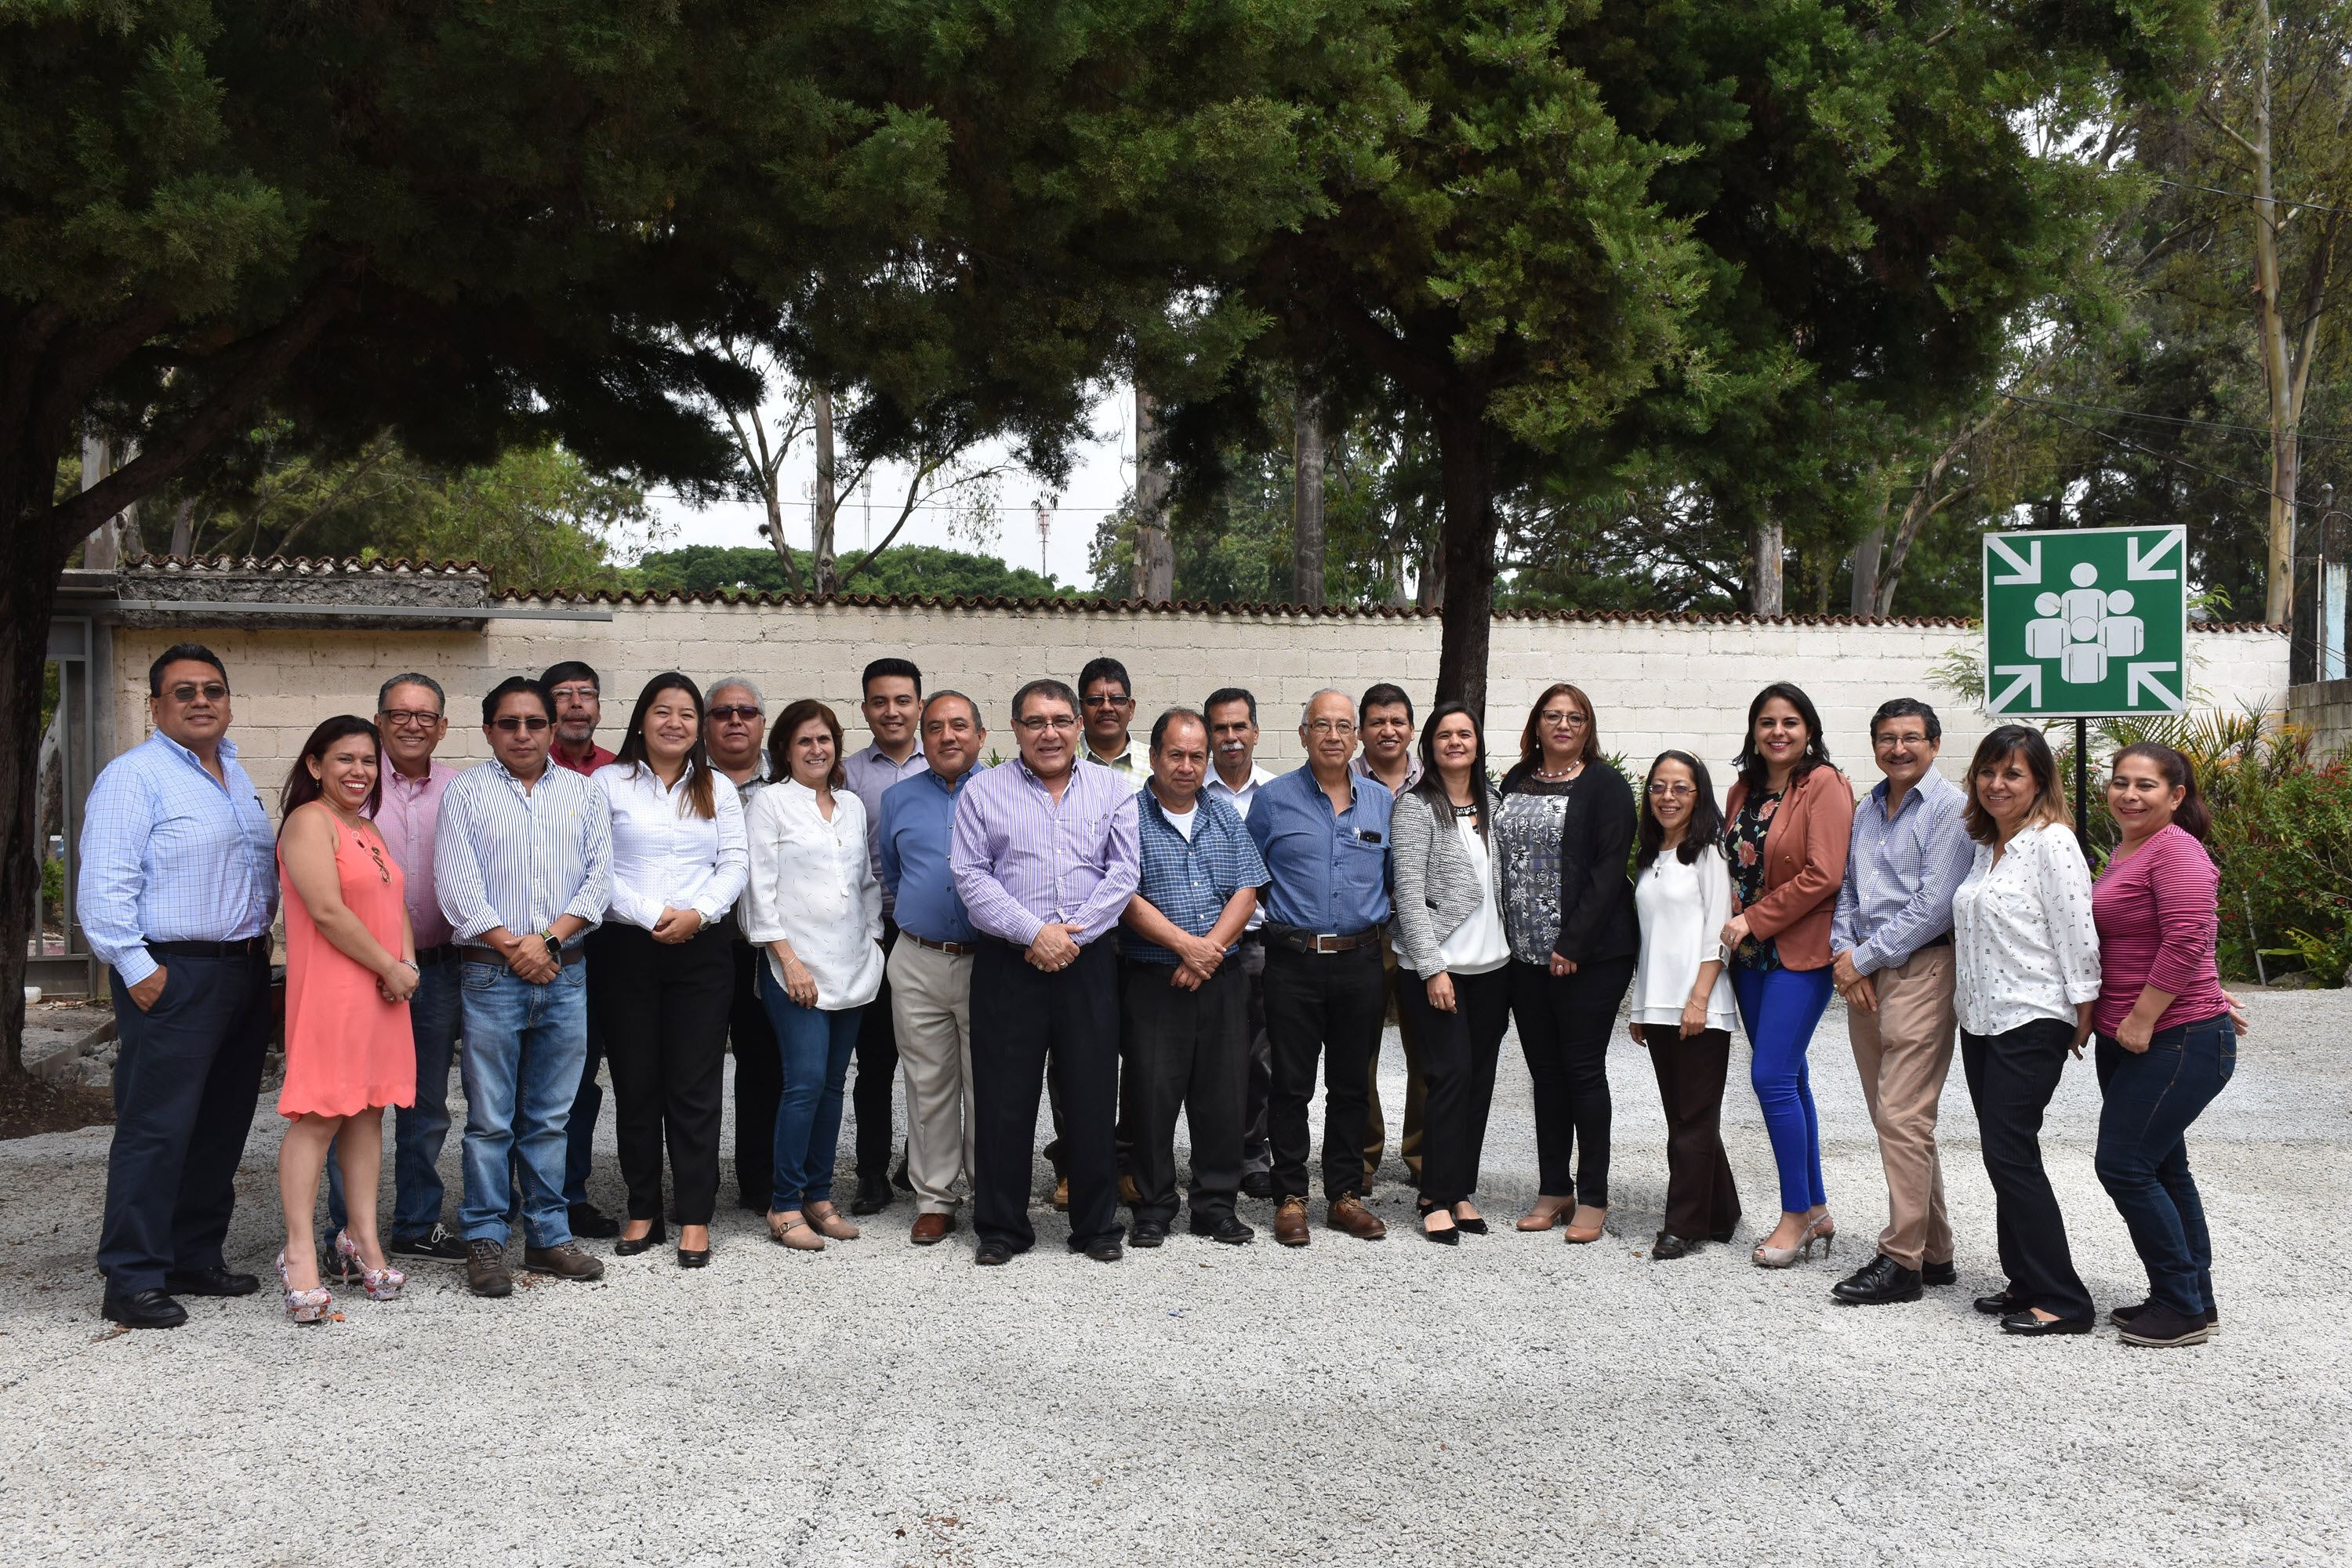
\includegraphics[width=0.67\linewidth]{images/201901-unidadeps-imagen02} 

}

\caption{Personal de Unidad de Prácticas de Ingeniería y Ejercicio Profesional Supervisado}\label{fig:unnamed-chunk-7}
\end{figure}

\begin {multicols}{2}

\hypertarget{descripcion-de-personal-administrativo-y-docente}{%
\subsection*{Descripción de Personal Administrativo y Docente}\label{descripcion-de-personal-administrativo-y-docente}}
\addcontentsline{toc}{subsection}{Descripción de Personal Administrativo y Docente}

A continuación nombres (Izquierda a Derecha):

\begin{itemize}
\item
  Ingeniero Mecánico Emilio Vladimir Lux Monroy
\item
  Ingeniera Industrial Yocasta Ivanobla Ortíz del Cid
\item
  Ingeniero Civil Silvio José Rodríguez Serrano
\item
  Ingeniero Electricista Natanael Jonathan Requena Gómez
\item
  Ingeniero Mecánico Carlos Anibal Chicojay Coloma
\item
  Ingeniera Industrial Sindy Massiel Godinez Bautista
\item
  Ingeniero Civil Manuel Alfredo Arrivillaga Ochaeta
\item
  Ingeniera Civil Christa del Rosario Classon de Pinto
\item
  Ingeniero Mecánico Diego Israel Navarro Godinez
\item
  Ingeniero en Ciencias y Sistemas Sergio Leonel Gómez Bravo
\item
  Ingeniero Civil Oscar Argueta Hernández
\item
  Ingeniero Mecánico Edwin Estuardo Sarceño Zepeda
\item
  Ingeniero Civil Luis Gregorio Alfaro Véliz
\item
  Ingeniero Electricista Francisco Javier Gonzalez López
\item
  Ingeniero Civil Juan Merck Cos
\item
  Ingeniero Químico Sergio Alejandro Recinos
\item
  Ingeniera Industrial Sigrid Alitza Calderón de León
\item
  Ingeniera Industrial Norma Ileana Sarmiento Zeceña de Serrano
\item
  Ingeniera Química Lorena Victoria Pineda Cabrera
\item
  Ingeniera Industrial Rocio Carolina Medina Galindo
\item
  Ingeniero Industrial Jaime Humberto Batten Esquivel
\item
  Ingeniera Civil Mayra Rebeca García Soria de Sierra
\item
  Licenciada en Administración de Empresas Maria Roxana Alvarado Monterroso
\end{itemize}

\end {multicols}

\hypertarget{jmerck}{%
\chapter{El Ejercicio Profesional Supervisado en la FIUSAC. Sus orígenes (I parte)}\label{jmerck}}

\begin {flushleft}

\begin{tcolorbox}[sharp corners=uphill, colback=fondo, colframe=fondo, arc=6mm, boxrule=0mm, boxsep=2mm,  opacityframe=0.19,  opacityback=0.19]

\begin{minipage}[c]{3cm}

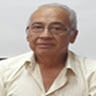
\includegraphics[width=2.5cm,height=\textheight]{images/201901-jmerck-photo.jpg}

\end{minipage}\begin{minipage}[c]{12cm}

\textbf{Autor:} \emph{Juan Merck Cos}\\
\textbf{Correo electrónico:} \emph{\href{mailto:juanmerck@gmail.com}{\nolinkurl{juanmerck@gmail.com}}}\\
\textbf{Fecha:} \emph{02 de mayo de 2019}

\end{minipage}

\end {tcolorbox}

\end {flushleft}

\begin {multicols*}{2}

\hypertarget{historia}{%
\section*{Historia}\label{historia}}
\addcontentsline{toc}{section}{Historia}

Como actividad académica, el Ejercicio Profesional Supervisado, EPS, es una proyección de la USAC, hacia la comunidad de nuestro país, que se realiza a través del programa de prácticas ligado a los planes de estudio, con el propósito de confrontar la teoría con la práctica en un campo real de aplicación. ¿Cómo? Atendiendo necesidades de servicios básicos, saneamiento, infraestructura de la industria, del sector eléctrico, económico, informático y de sistemas, y en general de índole tecnológico, planteando o proponiendo soluciones factibles a la problemática que se presenta, según sea el caso.

Esta práctica o actividad es realizada por estudiantes con cierre de pénsum, con la asesoría y supervisión de profesores que acompañan al estudiante, durante un periodo de 6 meses. El estudiante que decide realizar el EPS, (cabe aclarar que en la FIUSAC el EPS es optativo, a diferencia de otras facultades como Medicina, Odontología, Arquitectura, Agronomía, Veterinaria, entre otras, en las cuales sí es obligatorio), debe incorporarse a una institución que requiera del apoyo técnico.

¿Cómo nace la idea de realizar este tipo de actividades proyectadas hacia la sociedad? Fue en la Reforma de Córdova de 1918 que surge como una necesidad de que las universidades, principalmente las de carácter público, se vinculen con la sociedad a través de prácticas de extensión, de manera que el estudiante se involucre directamente con quienes padecen la problemática, permitiendo así conocer el medio hacia el cual va encaminada la propuesta de solución.

En la FIUSAC nace el EPS como una inquietud estudiantil, y fue a través de la Asociación de Estudiantes de Ingeniería, en los años 1971-1972, que con el impulso de un grupo de estudiantes idealistas, la junta directiva de la asociación creó la Secretaría de Extensión Universitaria, con el propósito de atender las solicitudes de comunidades del interior de la República, específicamente del área rural, de apoyo técnico para resolver problemas de agua potable, carreteras, infraestructura; en ese entonces eran exclusivamente del área de Ingeniería Civil.

Este servicio a la comunidad, por parte de la AEI fue incipiente, por la falta de apoyo oficial y no se diga de recursos, pero a la vez muy educador, por cuanto sentó las bases para que el programa de EPS surgiera como una necesidad dentro de la formación académica del futuro profesional de la Ingeniería. En este caso en particular se puede decir, que en la FIUSAC el EPS nace con una exigencia estudiantil de realizar prácticas extramuros, que sirviera como laboratorios para la futura práctica profesional, demandando para el efecto, que dentro del pénsum de estudio se incorporaran oficialmente estas prácticas.

Para llegar a lo que en la actualidad es el programa de EPS se tuvieron que superar muchos obstáculos de diferente índole, desde legales, administrativos e ideológicos; recordar que en ese entonces se vivía la época de la guerra fría; el sector docente se oponía al programa, ya que no compartían los beneficios que el mismo ofrecía dentro de la formación académica. Fue una lucha contra el sistema que imperaba, sin embargo, el sector más interesado, el estudiantil, tenía consciencia de lo que el programa representaba, por lo que lo apoyó e impulsó.

Un evento transcendental en la vida de nuestro país, que propició que el programa de EPS levantara vuelo como tal; fue el terremoto del año 1976, que evidenció las carencias que el país padecía y que la FIUSAC debía y tenía que atender. Fue así como se oficializó el programa de Prácticas y EPS, incorporándolo a los planes de estudio, las cuales hasta el día de hoy se siguen impartiendo, con muy buenos resultados, tanto para nuestra sociedad como para la formación académica y profesional del estudiante.

\end {multicols*}

\hypertarget{oargueta}{%
\chapter{Consejos para realizar una Buena Práctica Profesional}\label{oargueta}}

\begin {flushleft}

\begin{tcolorbox}[sharp corners=uphill, colback=fondo, colframe=fondo, arc=6mm, boxrule=0mm, boxsep=2mm,  opacityframe=0.19,  opacityback=0.19]

\begin{minipage}[c]{3cm}

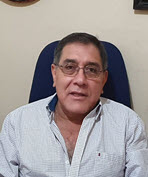
\includegraphics[width=2.5cm,height=\textheight]{images/201901-oargueta-photo.jpg}

\end{minipage}\begin{minipage}[c]{12cm}

\textbf{Autor:} \emph{Oscar Argueta Hernández}\\
\textbf{Correo electrónico:} \emph{\href{mailto:construcsjrs@yahoo.com}{\nolinkurl{construcsjrs@yahoo.com}}}\\
\textbf{Fecha:} \emph{09 de mayo de 2019}

\end{minipage}

\end {tcolorbox}

\end {flushleft}

\begin {multicols}{2}

La elección adecuada del lugar donde hará la práctica es el primer paso para el desarrollo de la carrera profesional. Es aquí en donde el estudiante conoce realmente el entorno del ambiente en que podrá desarrollarse para el futuro; allí podrá potenciar su conocimiento y verificar qué enfoque le dará a su labor profesional de acuerdo con sus intereses. Esta es la instancia más comprometida de su vida, pues conocerá todas las expectativas que puedan darse laboralmente, de acuerdo con su especialidad.

Para que el resultado de la práctica de ingeniería sea efectivo el estudiante debe orientarla en aquellas áreas en las que pueda desenvolverse con mayor acierto. La elección adecuada fortalecerá la iniciación apropiada en el mundo laboral, ya que es en este ambiente en donde podrá reconocer cuáles son sus habilidades y capacidades.

¿De qué manera podrá elegirse eficazmente el lugar donde se hará la práctica para optimizar los resultados? Algo muy importante es tener varias alternativas; las mismas están proyectadas por las diversas empresas o entidades que han hecho solicitud previa a la Unidad de EPS. Cualquier estudiante puede sentar las bases de un futuro laboral productivo a partir del desempeño que manifieste en la práctica.

Para la ejecución de una práctica eficiente con proyección a un futuro laboral exitoso, deben tomarse en cuenta los siguientes aspectos:

\begin{enumerate}
\def\labelenumi{\alph{enumi}.}
\item
  Buscar personalmente las oportunidades: si el futuro profesional advierte que en el EPS no se han presentado posibles escenarios para ejecutar la práctica, él mismo deberá de indagar en diferentes empresas, comunidades o entidades si ofrecen espacios laborales para la realización de su EPS. Es conveniente que el estudiante manifieste su interés y dé a conocer la oferta relacionada con su especialidad. De esa manera tendrá varias posibilidades y podrá seleccionar la que más se adapte a sus motivaciones.
\item
  Aprender de quien posee la experiencia: cuando se inicia la práctica existe temor de cometer algún error aunque se tenga el conocimiento previo; por tal razón es conveniente asimilar lo que dicen y hacen los expertos, pues son ellos quienes a través de la práctica han acumulado el conocimiento y pericia necesarios. Para obtener el éxito deseado en cualquier proyecto, el estudiante debe mostrar interés por aprender; esto se reflejará con la apropiación de la experiencia de otros.
\item
  Cumplir con responsabilidad las tareas asignadas: es en la práctica donde los empresarios podrán advertir el profesionalismo y el nivel de compromiso que adquiere el practicante. Esto puede conducir a una buena recomendación o su asimilación como parte del equipo de trabajo de la empresa o entidad.
\item
  Conocer claramente cuáles son las expectativas de la empresa: desde el inicio de la práctica el practicante debe manifestar interés en lo que la empresa o entidad aspira y requiere. Puede tratarse de un trabajo operativo o de algún cargo que requiera responsabilidad y control de mando; en ambos casos debe sacarse el mayor provecho posible.
\item
  La proactividad conlleva al liderazgo: un elemento clave que conlleva al liderazgo es que el practicante ejecute más de lo que se le requiere; si se tiene iniciativa de hacer más de lo solicitado, esto demostrará el compromiso que el epesista tiene con quienes le han cedido el espacio laboral para adquirir experiencia; este es un elemento clave que permitirá dejar huella en su desarrollo profesional.
\item
  Habilidad de trabajo en equipo y relaciones sociales: la convivencia laboral es importante para la obtención de un beneficio común y el éxito de la empresa o institución; pero también es importante que el practicante genere contacto con personeros de otras empresas o instituciones para extender el grado de participación de todos y compartir beneficios mutuos.
\item
  Proyectar el éxito con el tiempo: es necesario que el practicante se proyecte a futuro; qué es lo que se quiere ser u obtener dentro de 3, 5 o 10 años.
\item
  La retroalimentación como elemento básico para el éxito: el estudiante deberá verificar cuáles son los aspectos en que se puede mejorar en una empresa o institución; esto le permitirá transformar su proceder en acciones diversas. No obstante, los practicantes deben darse a conocer para encausar las tareas hacia la obtención del resultado deseado.
\item
  Reconocer que la práctica es el espacio temporal para demostrar las habilidades personales: aprovechar el período de práctica para manifestar la proactividad, conocimiento, compromiso, puntualidad y responsabilidad, ya que esto será el fundamento para su éxito profesional.
\end{enumerate}

\end {multicols}

\begin{center}\rule{0.5\linewidth}{\linethickness}\end{center}

\begin{figure}[H]

{\centering 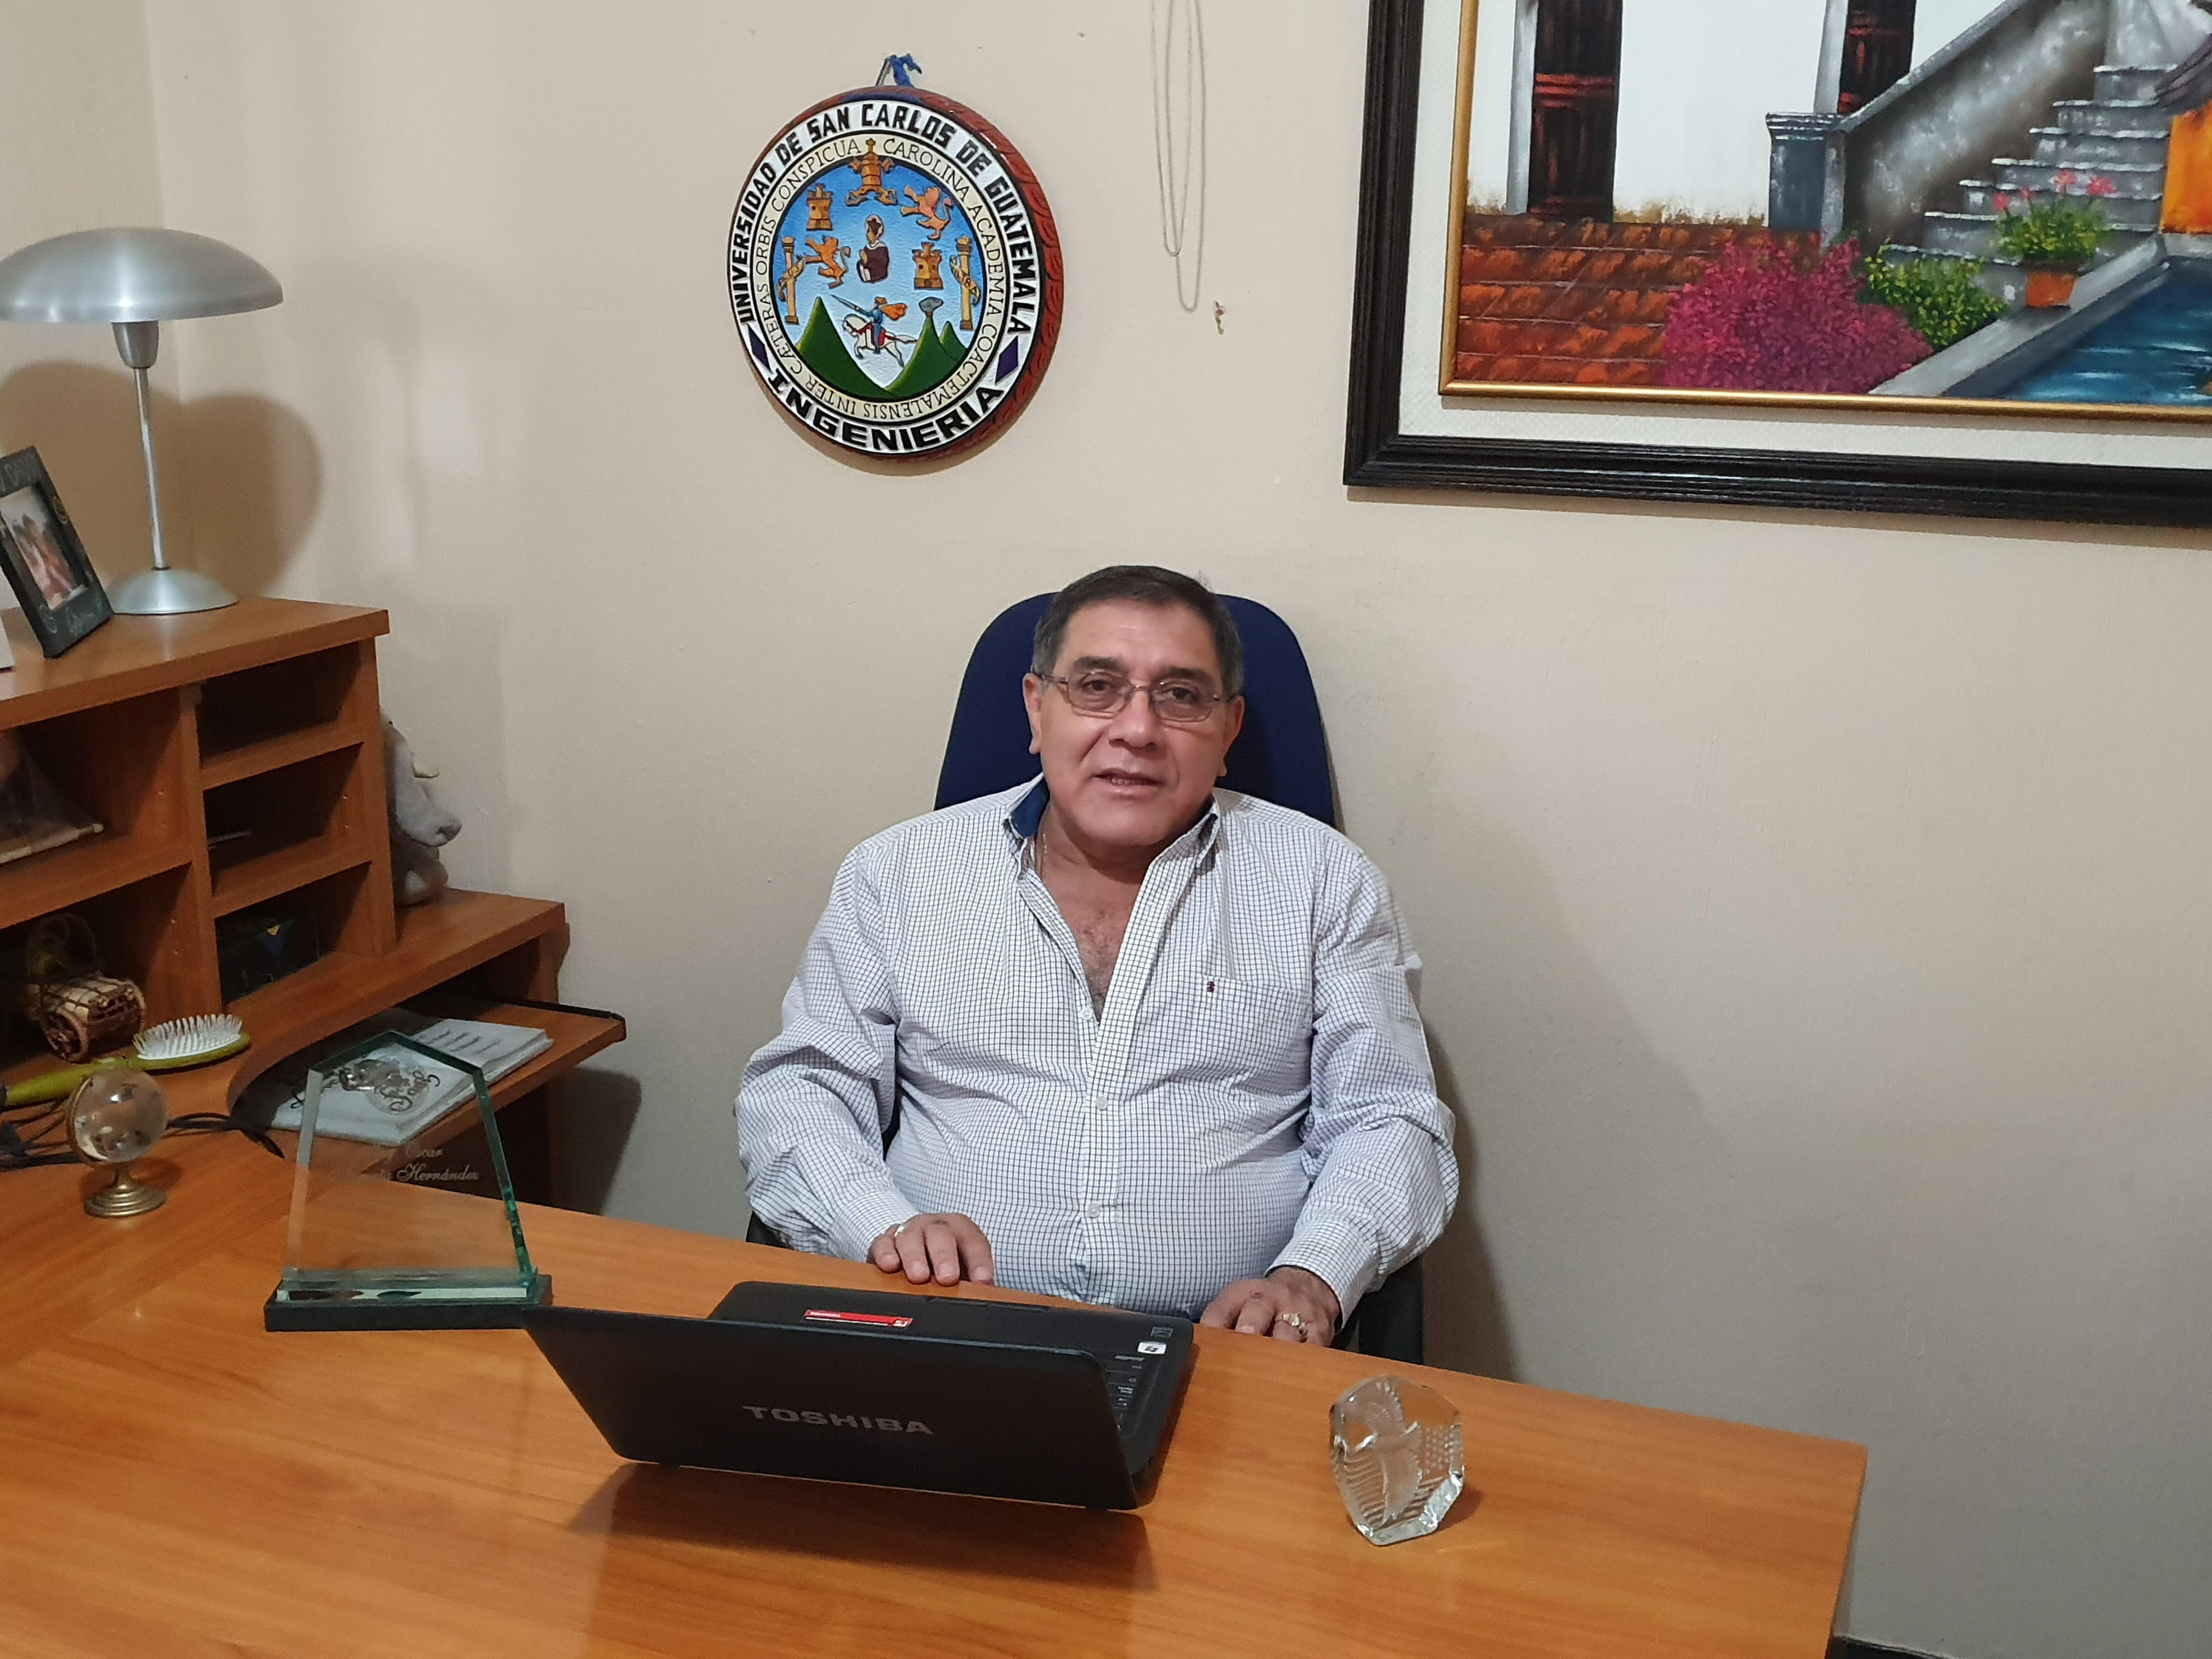
\includegraphics[width=0.8\linewidth]{images/201901-oargueta-imagen01} 

}

\caption{Ing. Oscar Argueta}\label{fig:unnamed-chunk-8}
\end{figure}

\hypertarget{bfuentes}{%
\chapter{Mejores prácticas para un EPS Exitoso}\label{bfuentes}}

\begin {flushleft}

\begin{tcolorbox}[sharp corners=uphill, colback=fondo, colframe=fondo, arc=6mm, boxrule=0mm, boxsep=2mm,  opacityframe=0.19,  opacityback=0.19]

\begin{minipage}[c]{3cm}

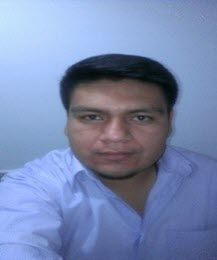
\includegraphics[width=2.5cm,height=\textheight]{images/201901-bfuentes-photo.jpg}

\end{minipage}\begin{minipage}[c]{12cm}

\textbf{Autor:} \emph{Bryan Otto Fuentes Paz}\\
\textbf{Correo electrónico:} \emph{\href{mailto:bryan.fuentespaz@gmail.com}{\nolinkurl{bryan.fuentespaz@gmail.com}}}\\
\textbf{Fecha:} \emph{27 de marzo de 2019}

\end{minipage}

\end {tcolorbox}

\end {flushleft}

\hypertarget{resumen}{%
\section*{Resumen}\label{resumen}}
\addcontentsline{toc}{section}{Resumen}

El presente artículo trata sobre mi experiencia como asesor de proyectos de EPS; describo algunos factores que deben tomarse en cuenta para que el proyecto sea exitoso, así como la importancia que estos tienen para el crecimiento tecnológico de las instituciones que se ven involucradas en el proceso. También hago referencia al impacto que tiene la colaboración y el intercambio de conocimiento para solucionar problemas empleando la tecnología, concluyendo que los trabajos de EPS son beneficiosos al no tener un costo directo, ya que se aprovecha la cooperación interinstitucional.

\hypertarget{abstract}{%
\section*{Abstract}\label{abstract}}
\addcontentsline{toc}{section}{Abstract}

This article deals with my experience as an EPS Project Advisor, I describe some factors that must be taken into account in order for the project to be successful, as well as the importance that these have for the technological growth of the institutions that are involved in the process. I also refer to the impact of the collaboration and the exchange of knowledge to solve problems using technology, concluding that EPS works are beneficial because they do not have a direct cost and take advantage of inter-institutional cooperation.

\hypertarget{palabras-clave}{%
\section*{Palabras Clave:}\label{palabras-clave}}
\addcontentsline{toc}{section}{Palabras Clave:}

\emph{Ejercicio Profesional Supervisado, EPS, USAC, Asesoría.}

\begin {multicols}{2}

\hypertarget{introduccion-1}{%
\section{Introducción}\label{introduccion-1}}

La Universidad de San Carlos de Guatemala, siendo la rectora de la educación superior en Guatemala, debe estar siempre a la vanguardia y para ello es necesario invertir en tecnología y en recurso humano que permita lograr proyectos de alto impacto que faciliten la enseñanza-aprendizaje; así como mejorar los procesos administrativos y la gobernanza en el sistema educativo que establezca estándares de alta calidad. Estas condiciones generan un ecosistema para promover y fortalecer los lazos interinstitucionales que permitan concebir estrategias y plataformas tecnológicas para resolver problemas de nuestra sociedad, siendo esto una clara oportunidad para los proyectos de extensión.

\hypertarget{articulo}{%
\section{Artículo}\label{articulo}}

En el Artículo 2º del Capítulo I del Normativo del Ejercicio Profesional Supervisado de Graduación (EPS FINAL) de la Facultad de Ingeniería de la Universidad de San Carlos de Guatemala, se define EPS Final como: ``las actividades académicas de docencia-aprendizaje, investigación y de servicio técnico profesional universitario que los estudiantes con cierre de pénsum de estudios realizan en el medio real del país, para desarrollar proyectos relativos a su profesión''.

La labor que realiza un asesor es importante para encaminar un proyecto y que el mismo pueda ser exitoso; sin embargo no debe tomarse a la ligera, ya que, al mismo tiempo que se desarrolla una solución tecnológica, también se forma una experiencia real en el estudiante.

En varias ocasiones el proyecto de EPS suele ser un primer contacto con el ámbito laboral que tiene un estudiante, es por ello que el conocimiento y seguimiento que un asesor brinda debe ser integral.

El vínculo asesor-estudiante debe ser estrecho para lograr una buena comunicación y fluidez en cada etapa del proyecto.

En mi experiencia como asesor de la Escuela de Ciencias y Sistemas de la Facultad de Ingeniería, para proyectos de Ejercicio Profesional Supervisado (EPS), se han podido identificar algunos factores que permiten que un proyecto pueda ser exitoso y que logre tener un impacto significativo para la población objetivo:

\begin{itemize}
\item
  Una correcta toma e interpretación de requerimientos: en todo proyecto es vital conocer las necesidades que se quieren cubrir en la institución que se realiza el EPS, para lo cual es conveniente indagar y extraer todas las características fundamentales de los procesos que quieren ser automatizados; si la interpretación es correcta entonces se puede dar una solución tecnológica correcta.
\item
  Compromiso institución-estudiante-asesores: debe existir un compromiso tangible entre cada uno de los actores para que los proyectos puedan ser finalizados, implementados y autosostenibles, el desinterés de cualquiera de ellos es un riesgo alto para que el proyecto fracase.
\item
  Infraestructura: es importante que la institución posea la infraestructura adecuada para la implementación y despliegue de la solución tecnológica, para que esta pueda ser aprovechada al máximo.
\item
  Difusión de procesos automatizados: la difusión logra que los procesos sean conocidos y brinden una plataforma, para que exista una aceptación integral de las nuevas formas de realizarlos.
\item
  Capacitación a usuarios finales: la capacitación es el proceso educativo a corto plazo que permite la correcta formación de los colaboradores para la utilización de soluciones tecnológicas y conocimiento de los procesos, esto les brinda la capacidad de desempeñarse de mejor manera en sus puestos laborales.
\item
  Soporte técnico (período de gracia): el período de gracia como soporte tiene la intención de que las soluciones tecnológicas estén libres de errores y, por lo tanto, logren que funcionen correctamente sin causar incidencias en los procesos.
\item
  Recepción del proyecto de EPS por parte del departamento de tecnología o departamento afín: para que un proyecto pueda permanecer y ser autosostenible es necesario que al momento de concluir el EPS, este quede a cargo del departamento de tecnología para su mejora y expansión.
\end{itemize}

He tenido la oportunidad de asesorar proyectos de EPS, mismos que han sido concluidos de manera exitosa gracias al cumplimiento de los factores antes mencionados. Cada uno de los proyectos ha sido ejecutado siguiendo estándares y niveles de servicio aptos para un alto rendimiento; algunos de ellos puestos a prueba bajo situaciones complejas y exigentes.

Recientemente fue condecorado el Ingeniero en Ciencias y Sistemas Rodrigo Antonio Herrera de León con el premio Francisco Vela 2018, por la excelencia de su trabajo de graduación titulado: Automatización del módulo de recuperación en la Oficina de Control Académico, Facultad de Humanidades, Universidad de San Carlos de Guatemala, epesista al cual tuve la oportunidad de asesorar.

Personalmente considero que el beneficio obtenido gracias a los proyectos de EPS es superior a cualquier inversión que pueda hacerse para ejecutarlos; en primer lugar porque no existe un costo directo pues el estudiante no recibe remuneración alguna; en segundo lugar las inversiones generan mejoras en los procesos y avances tecnológicos para facilitarlos y beneficiar a la población objetivo.

\end {multicols}

\begin{figure}[H]

{\centering 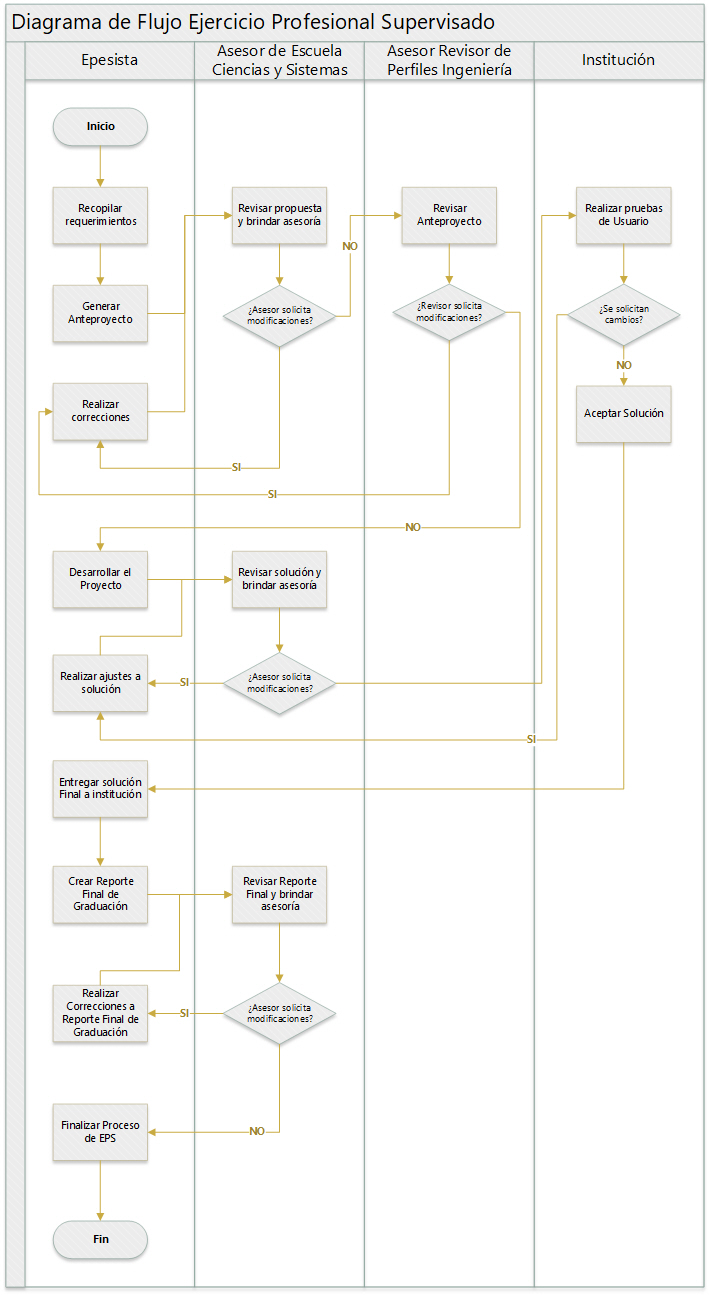
\includegraphics[width=0.7\linewidth]{images/201901-bfuentes-image01} 

}

\caption{Diagrama de Flujo EPS}\label{fig:unnamed-chunk-9}
\end{figure}

\begin {multicols}{2}

\hypertarget{conclusiones}{%
\section{Conclusiones}\label{conclusiones}}

\begin{itemize}
\item
  La importancia de los proyectos de EPS radica en el impacto y beneficio para la población objetivo, que puede lograrse gracias a la colaboración entre institución-estudiante y la correcta asesoría tanto técnica como de la propia institución en donde se ejecuta el proyecto.
\item
  Ser parte del proceso de asesoría de proyectos de EPS es una experiencia enriquecedora y una oportunidad para contribuir con la solución de problemas en nuestra sociedad a través de la tecnología.
\item
  La automatización de los procesos genera cambios notorios tanto en la reducción del tiempo que toma concluirlos, como en el correcto aprovechamiento de los recursos.
\item
  La mejora continua en el proceso de proyectos de EPS contribuye con el desarrollo oportuno y estándares de calidad de las soluciones tecnológicas que el epesista puede desarrollar y ejecutar.
\item
  El contacto con problemas reales le brinda al epesista una experiencia que permite un crecimiento integral.
\end{itemize}

\hypertarget{referencias}{%
\section{Referencias}\label{referencias}}

\begin{itemize}
\item
  Departamento de EPS. Facultad de Ingeniería. USAC. (2006). \emph{Normativo del Ejercicio Profesional Supervisado de Graduación (EPS FINAL) de la Facultad de Ingeniería de la Universidad de San Carlos de Guatemala\footnote{\url{https://portal.ingenieria.usac.edu.gt/reglamentos/NormativoEPS.pdf}}} {[}Consulta en línea: 2019{]}.
\item
  HERRERA DE LEÓN, Rodrigo Antonio. (2017). \emph{Automatización del módulo de recuperación en la oficina de Control Académico, Facultad de Humanidades, Universidad de San Carlos de Guatemala\footnote{\url{http://www.repositorio.usac.edu.gt/8239/1/Rodrigo} Antonio Herrera De León.pdf}.} {[}Consulta en línea: 2019{]}.
\end{itemize}

\end {multicols}

\hypertarget{gfong}{%
\chapter{Tratamiento de los Desechos y su Aprovechamiento en la Generación de Energía Eléctrica}\label{gfong}}

\begin {flushleft}

\begin{tcolorbox}[sharp corners=uphill, colback=fondo, colframe=fondo, arc=6mm, boxrule=0mm, boxsep=2mm,  opacityframe=0.19,  opacityback=0.19]

\begin{minipage}[c]{3cm}

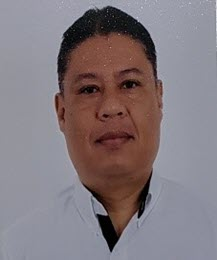
\includegraphics[width=2.5cm,height=\textheight]{images/201901-gfong-photo.jpg}

\end{minipage}\begin{minipage}[c]{12cm}

\textbf{Autor:} \emph{Gabriel Fong Mazariegos}\\
\textbf{Correo electrónico:} \emph{\href{mailto:director@guateverde.com.gt}{\nolinkurl{director@guateverde.com.gt}}}\\
\textbf{Fecha:} \emph{29 de abril de 2019}

\end{minipage}

\end {tcolorbox}

\end {flushleft}

\hypertarget{resumen-1}{%
\section*{Resumen}\label{resumen-1}}
\addcontentsline{toc}{section}{Resumen}

El presente trabajo se basa en el estudio de la cantidad de los desechos sólidos orgánicos y de las aguas residuales del tipo ordinario, generados por los habitantes de la cabecera departamental de Jutiapa, con la finalidad de darle un tratamiento adecuado, y así determinar su potencial y aprovechamiento como biomasa en el proceso de biodigestión, para lo cual se utiliza un biodigestor que se encarga de procesar la materia orgánica presente tanto en los desechos sólidos, como en el agua residual del tipo ordinaria.

Con este proceso de tratamiento se espera obtener dos subproductos, los cuales serán reutilizables posteriormente;, el primero consiste en la obtención de biogás, un gas compuesto básicamente por metano, dióxido de carbono, y en menor cantidad sulfuro de hidrógeno, oxígeno y nitrógeno, el cual puede usarse como combustible en aplicaciones como: la sustitución del gas propano o LPG en procesos que así lo requieran, tales como calderas, sistemas de calefacción y estufas de uso doméstico o industrial; también puede utilizarse como combustible en el proceso de generación de energía eléctrica, a través de generadores eléctricos accionados por motores de combustión interna; este gas sustituye al combustible fósil utilizado frecuentemente, en la generación de energía eléctrica como: gasolina, diésel, bunker o querosén. El segundo subproducto es un agua tratada que contiene nitrógeno, fósforo y potasio, que actúa como fertilizante y mejoradora de suelos en procesos de fertirriego; se puede utilizar para cierta clase de cultivos como: caña de azúcar y maíz, así como para consumo animal, café, árboles frutales, pastos, entre otros.

\hypertarget{abstract-1}{%
\section*{Abstract}\label{abstract-1}}
\addcontentsline{toc}{section}{Abstract}

The present work is based on the study of the amount of organic solid waste and wastewater of the ordinary type, generated by the inhabitants of the departmental capital of Jutiapa, in order to give it an adequate treatment, and thus to determine its potential and use as biomass, in the process of biodigestion, for which a biodigester is used that is responsible for processing the organic matter present in both solid waste as well as waste water of the ordinary type.

\newpage

With this process of treatment, it is expected to obtain two byproducts which will be reusable later, the first one consists in obtaining biogas, a gas composed basically of methane, carbon dioxide, and in less amount of hydrogen sulfide, oxygen, nitrogen, which can be used as fuel in applications such as: the replacement of propane gas or LPG, in processes that require it, among which we find, boilers, heating systems and stoves for domestic or industrial use, we can also use it as fuel in the process of electric power generation, through electric generators powered by internal combustion engines, this gas replaces the fossil fuel used frequently, in the generation of electric power such as: gasoline, diesel, bunker or kerosene. The second by-product, is a treated water that contains nitrogen, phosphorus and potassium, which acts as fertilizer and soil improver in fertigation processes, and can be used for certain kinds of crops such as: sugar cane, corn for animal consumption, coffee, fruit trees, pastures, etc.

\hypertarget{palabras-clave-1}{%
\section*{Palabras Clave:}\label{palabras-clave-1}}
\addcontentsline{toc}{section}{Palabras Clave:}

\emph{Desechos sólidos orgánicos, aguas residuales ordinarias, biodigestor, biogás, fertirriego.}

\begin {multicols}{2}

\hypertarget{introduccion-2}{%
\section{Introducción}\label{introduccion-2}}

Hasta hace unos años, el tema de tratamiento de desechos sólidos orgánicos y aguas residuales en Guatemala, era para muchos un gasto, que solamente elevaba los costos de producción para el caso de la industria; para las instituciones de gobierno como las municipalidades, significaba una reducción en los ingresos y la limitante de ejecutar una mayor cantidad obras públicas.

Hoy en día existen alternativas que permiten, no solo darle un tratamiento a este tipo de desechos, sino que además sacarle provecho; uno de estos procesos consiste en la utilización de un sistema de biodigestión, llamado biodigestor que no es más que una cámara hermética donde se acumulan residuos orgánicos (vegetales, excremento de animales, aguas residuales ordinarias) mediante un proceso natural de bacterias (anaerobias) presentes en los excrementos que descomponen el material contenido en biogás y en fertilizante. Este biogás puede utilizarse como combustible en un motor de combustión interna, el que a su vez se acopla a un generador eléctrico, para posteriormente generar energía eléctrica que puede ser reutilizada en diferentes procesos o bien ser inyectada a la red de energía eléctrica nacional; por último se puede usar el fertilizante producido ya que contiene nitrógeno, fósforo y potasio, además de una carga bacteriana que permite no solo mejorar las propiedades del suelo, sino que ayudan a ciertos cultivos a desarrollarse de mejor manera.

\hypertarget{articulo-1}{%
\section{Artículo}\label{articulo-1}}

\hypertarget{produccion-de-desechos-solidos}{%
\subsection{Producción de desechos sólidos}\label{produccion-de-desechos-solidos}}

La cabecera departamental de Jutiapa no cuenta con una planta de tratamientos de desechos sólidos, por lo que la disposición final se realiza en un vertedero o relleno sanitario, el cual está ubicado en las afueras del casco urbano, en la finca El Estoraque; es arrendado por la municipalidad.

Actualmente estos desechos sólidos crecen, a medida que la población también lo hace, por lo tanto en la siguiente gráfica se ejemplifica cómo los habitantes de la cabecera departamental de Jutiapa contribuyen actualmente de manera directa a la generación de estos desechos sólidos, y el crecimiento proyectado de lo que se espera en los próximos años.

\begin {flushleft}
\noindent\begin{minipage}[c]{\columnwidth}

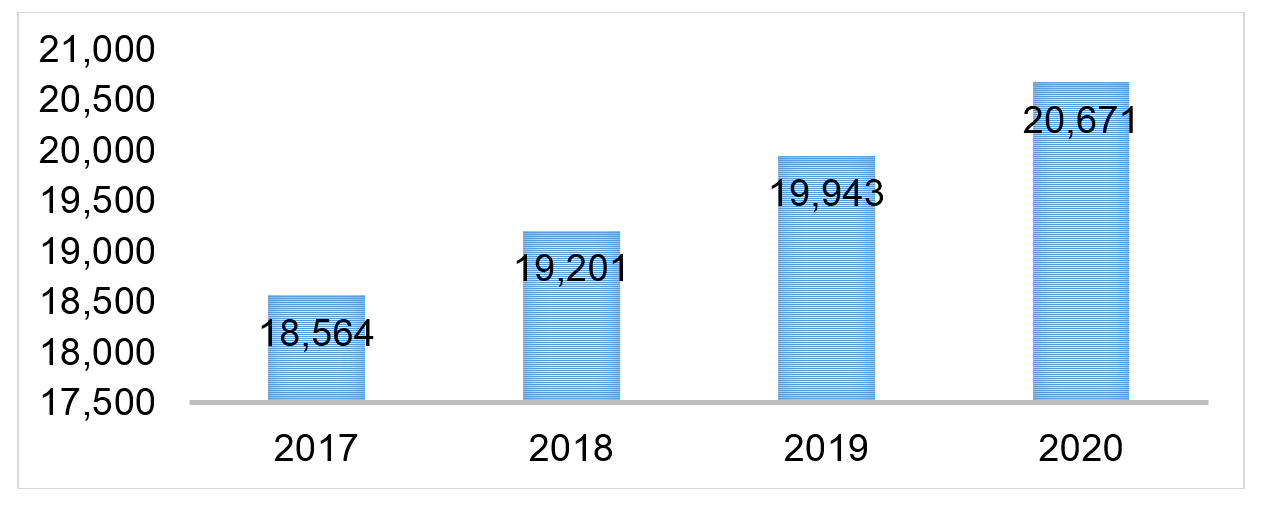
\includegraphics[width=1\linewidth]{images/201901-gfong-imagen01}
\figcaption{Proyección toneladas por año desechos sólidos}

\end{minipage}

\end {flushleft}

La población actual de Jutiapa cuenta con 41,847 habitantes, aproximadamente, los cuales residen en 8,369 hogares; parte de estos desechos sólidos recolectados son el producto de 2,000 hogares que representan el 23.89\% del total que pagan el servicio a la Asociación de Recolectores de basura de Jutiapa.

El resto de los hogares, que son 6,369, envían su basura a los dos centros de acopio ubicados; uno en el mercado central y el otro en el antiguo campo de la feria; así como en basureros clandestinos y la basura que se encuentra en calles y avenidas del casco urbano, la cual es recolectada por el Departamento de Mantenimiento Municipal. Esto representa el 76.10\% de los hogares; la cantidad de basura recolectada, según los centros de acopio, se refleja en la siguiente gráfica.

\begin {flushleft}
\noindent\begin{minipage}[c]{\columnwidth}

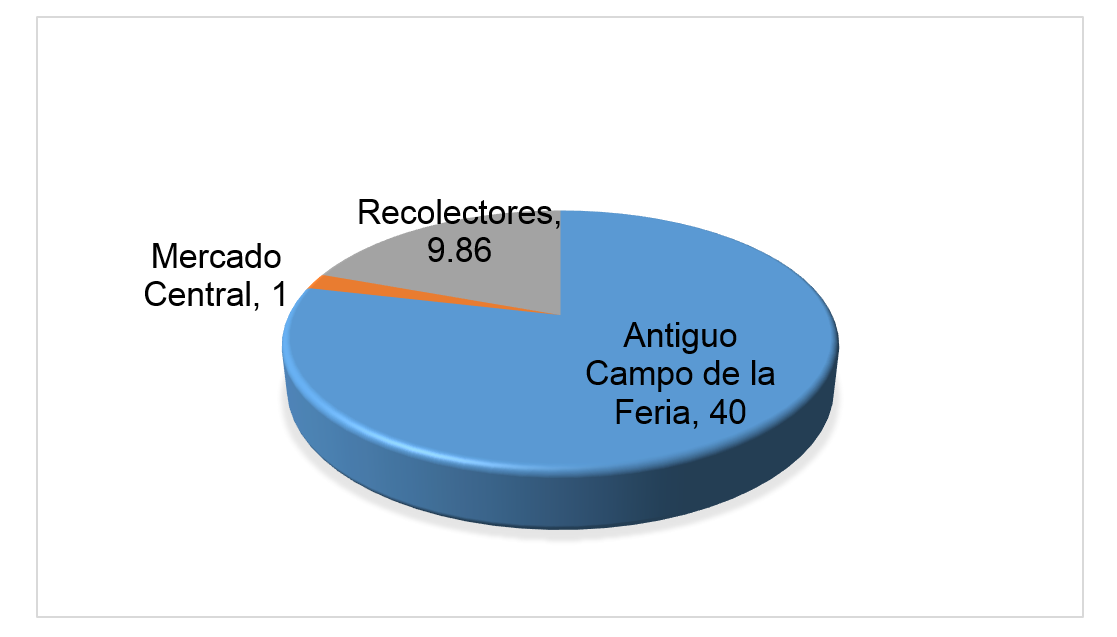
\includegraphics[width=1\linewidth]{images/201901-gfong-imagen02}
\figcaption{Cantidad de desechos recibida por día; Total 50.86 toneladas}

\end{minipage}

\end {flushleft}

En pruebas de campo se determinó que en un metro cúbico caben 33 bolsas negras estándar de basura, con un peso de 407 libras, de las cuales 363 son de desechos sólidos orgánicos (89.18 \%), mientras que el restante, 44 libras, son materiales inorgánicos que se pueden reciclar; por ejemplo: cartón, vidrio, plástico, bolsas de nylon, entre otros.

\hypertarget{produccion-de-aguas-residuales-ordinarias}{%
\subsection{Producción de aguas residuales ordinarias}\label{produccion-de-aguas-residuales-ordinarias}}

Las aguas residuales ordinarias son el producto de procesos comunes y cotidianos en los hogares, que van desde ducharse, usar el servicio sanitario, limpieza e higiene del hogar, entre otros. En algunos casos, las aguas residuales se recolectan, tratan y descargan por medio de un sistema común. En el municipio de Jutiapa, el sistema municipal no cuenta con una planta de tratamiento oficial y los drenajes se vierten directamente a los ríos o son conducidas al exterior de los hogares; sin embargo, en el casco urbano se cuenta con un nivel de tratamiento primario que consiste en eliminar los desechos sólidos de las aguas contaminadas de las fosas sépticas y al momento que desemboquen en los ríos La Paz, De La Virgen, Colorado y río Salado, reducen el nivel de contaminación.

Según el INE 2002, el 49.6\% de los hogares contaban con un servicio sanitario y el 36.24\% con fosas sépticas, excusados lavables y letrinas. Es de indicar que la red de drenajes abarcaba solamente al 20\% de los hogares y el 16.24 \% no contaba con algún servicio. (Diagnóstico socioeconómico, potencialidades productivas y propuestas de inversión, Facultad de Ciencias Económicas USAC, 2013, página 96).

Actualmente el sistema de alcantarillado Municipal, que recorre la cabecera departamental de Jutiapa, descarga en doce puntos diferentes, a lo largo de los ríos ya mencionados con anterioridad, los cuales fueron identificados y posicionados en el siguiente cuadro.

\begin {flushleft}
\noindent\begin{minipage}[c]{\columnwidth}

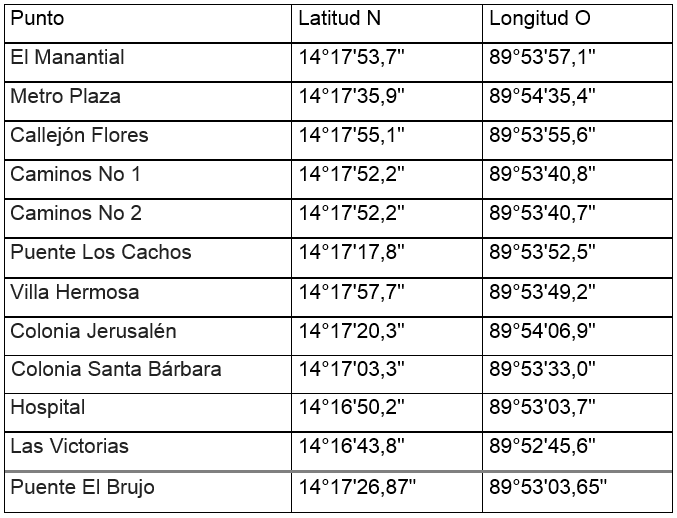
\includegraphics[width=1\linewidth]{images/201901-gfong-imagen03}
\figcaption{Coordenadas geográficas de puntos de monitoreo}

\end{minipage}

\end {flushleft}

Estos mismos 41,847 habitantes, aproximadamente, que residen en 8,369 hogares, generan los siguientes caudales de agua residual, vertidos en doce puntos diferentes.

\begin {flushleft}
\noindent\begin{minipage}[c]{\columnwidth}

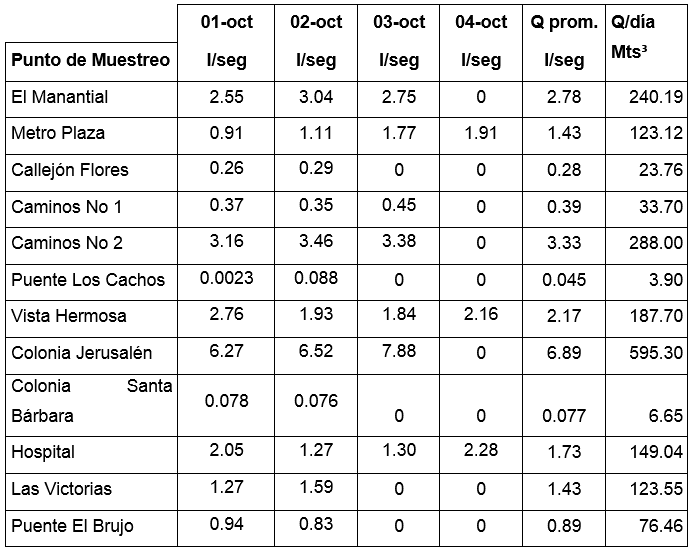
\includegraphics[width=1\linewidth]{images/201901-gfong-imagen04}
\figcaption{Medición de caudales en litros por segundo y metros cúbicos por día}

\end{minipage}

\end {flushleft}

\hypertarget{diseno-del-sistema-de-tratamiento}{%
\subsection{Diseño del sistema de tratamiento}\label{diseno-del-sistema-de-tratamiento}}

Como ya se dijo, este sistema es innovador porque combina un sistema tradicional de planta de tratamiento con uno anaeróbico (biodigestor), por lo que permite, entre otras cosas, aprovechar la materia orgánica y producir energía eléctrica, sumado a esto darle el tratamiento adecuado de las aguas residuales y basura, ya que hoy en día no se hace y por eso vemos focos de contaminación, y nuestros ríos y lagos agonizando por el alto grado de contaminación que reciben.

Por primera vez se habla de un sistema que puede generar ingresos económicos y ayudar de manera directa a la reducción de gases de efecto invernadero, causantes del cambio climático que actualmente vivimos; esto porque se atrapa y quema el gas metano producido durante la degradación de la materia orgánica presente en la basura y agua residual, y la reutilización del agua tratada para riego en los campos de siembra.

El sistema consta de las siguientes etapas o unidades:

\textbf{Tratamiento primario}

\begin{enumerate}
\def\labelenumi{\alph{enumi}.}
\item
  Caja de demasías
\item
  Canal de ingreso, rejas y desarenador
\item
  Plataforma para descarga de desechos
\item
  Tanque de captación
\end{enumerate}

\textbf{Tratamiento secundario}

\begin{enumerate}
\def\labelenumi{\alph{enumi}.}
\setcounter{enumi}{4}
\tightlist
\item
  Biodigestor
\end{enumerate}

\textbf{Tratamiento terciario}

\begin{enumerate}
\def\labelenumi{\alph{enumi}.}
\setcounter{enumi}{5}
\item
  Clarificador
\item
  Clorador
\item
  Tanque de contacto
\item
  Laguna secundaria
\item
  Toma para fertiriego
\end{enumerate}

Y de acuerdo con los desechos sólidos orgánicos y aguas residuales tratadas, se producirá lo siguiente:

1 tonelada de desecho sólido equivale a 66.15 mts³ de biogás, a una DQO de 5,500 mgl.

\hypertarget{desechos-solidos-organicos}{%
\subsection{Desechos sólidos orgánicos:}\label{desechos-solidos-organicos}}

La estimación de la cantidad de biogás a producir obedece al estudio realizado en un biodigestor del tipo propuesto en este proyecto, en él se ingresaron diferentes tipos de desechos sólidos orgánicos y se evaluaron durante un año; de ahí el factor de 66.15 mts³ de biogás por tonelada ingresada.

\begin {flushleft}
\noindent\begin{minipage}[c]{\columnwidth}

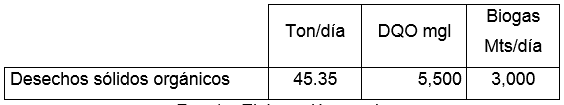
\includegraphics[width=1\linewidth]{images/201901-gfong-imagen05}
\figcaption{Valores de producción de biogás por tonelada de desecho sólidos}

\end{minipage}

\end {flushleft}

\hypertarget{agua-residual-tipo-ordinaria}{%
\subsection{Agua residual tipo ordinaria}\label{agua-residual-tipo-ordinaria}}

\begin {flushleft}

DQO Kg/día = (Q (m³/día) x DQO mgl)/1,000\\
Q = caudal por día medido en metros cúbicos.\\
DQO, Demanda Biológica de Oxígeno en miligramos por litro\\
DQO = (1,856.38 X 156.7) / 1,000 = 290.11 Kg.

\noindent\begin{minipage}[c]{\columnwidth}

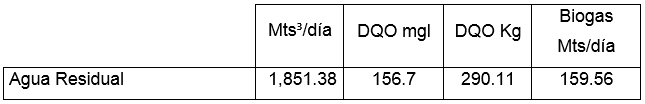
\includegraphics[width=1\linewidth]{images/201901-gfong-imagen06}
\figcaption{Producción de biogás por metro cúbico de agua residual}

\end{minipage}

\end {flushleft}

Para el caso del agua residual, por cada kilogramo de DQO se obtiene un factor de 0.55 mts³ de biogás; el factor se obtiene luego de realizar diferentes evaluaciones en sistema similar al propuesto para este caso, el valor de DQO corresponde a las mediciones realizadas durante 4 días en cada uno de los doce puntos de descarga.

Por lo tanto para el presente caso se tendrá una producción de biogás, equivalente a \textbf{3,159.56 mts³ por día}; este biogás equivale a 31.59 cilindros de 100 lbs de gas propano por día, o 322.40 gls de diésel por día, y 1,856.38 m³ de agua tratada para fertirriego.

Por lo tanto este biogás producido nos permite generar 250 Kwh por medio de un generador previamente arreglado para utilizar el biogás como combustible, durante 20 horas por día los 365 días del año, y tomando en cuenta el costo de implementación del proyecto, operación, mantenimiento y los ingresos extras por cobro de tratamiento de aguas residuales y basura orgánica, se tiene el siguiente cuadro.

\begin {flushleft}
\noindent\begin{minipage}[c]{\columnwidth}

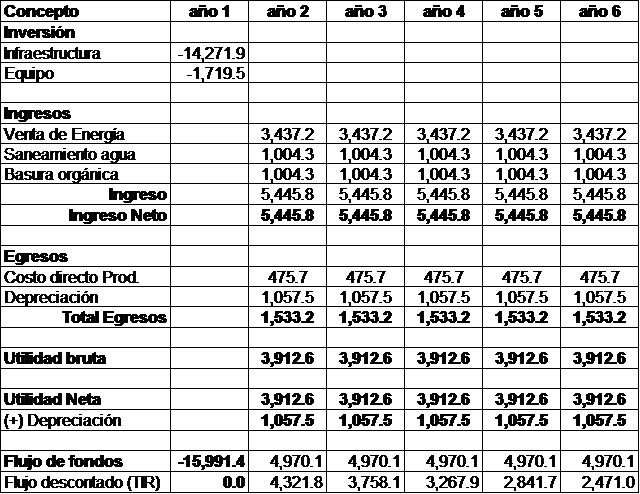
\includegraphics[width=1\linewidth]{images/201901-gfong-imagen07}
\figcaption{Flujo de fondos proyectado a 5 años; cifras en miles de quetzales}

\end{minipage}

\end {flushleft}

Se toma en cuenta una tasa de rendimiento del 15\%, la cual está conformada de la siguiente manera: 10\% que corresponde a la tasa a la cual el INFOM le presta a la municipalidad el dinero para realizar el proyecto, y 5\% de tasa de inflación anual según el Banco de Guatemala (año 2017).

Realizando los cálculos respectivos se tienen los siguientes indicadores financieros:

\begin{itemize}
\tightlist
\item
  Una valor actual neto (VAN) de Q 669,120.00
\item
  Tasa interna de retorno (TIR) 16.7539\%
\item
  Un período de recuperación de 4.875 años, es decir 4 años 8 meses y 23 días.
\end{itemize}

Como se ha venido explicando desde el inicio, el proyecto no solo cumple con el tratamiento de los desechos orgánicos sino que además genera ingresos; por primera vez se habla de un proyecto de tratamiento rentable, eficiente y amigable con el medio ambiente.

\hypertarget{conclusiones-1}{%
\section{Conclusiones}\label{conclusiones-1}}

\begin{itemize}
\item
  La propuesta y estudio de este Ejercicio Profesional Supervisado obedecen a 15 años de investigación y desarrollo propio, con 16 proyectos desarrollados y una potencia instalada en generación de energía eléctrica con biogás de 1.1 Mw.
\item
  Es posible proponer un sistema confiable para el tratamiento de las aguas residuales y desechos sólidos orgánicos, que salga de los sistemas tradicionales usados hasta el día de hoy en Guatemala.
\item
  Con las nuevas regulaciones de ley, en materia de tratamiento de aguas residuales y desechos sólidos, las municipalidades no han invertido en el cumplimiento de dichas regulaciones debido al costo de inversión de los sistemas convencionales de tratamiento, y las pocas que lo hacen terminan abandonándolos debido a su costo de operación.
\item
  El sistema de biodigestión permite capturar el gas metano 21 veces más contaminante que el dióxido de carbono, lo que hace el proyecto candidato para fuentes de financiamiento externas, pues contribuye a disminuir los gases de efecto invernadero, que a su vez es causante del cambio climático.
\item
  Debido a las características del sistema de tratamiento y la generación de energía eléctrica, el capital de inversión puede ser recuperado en período de 4 años 8 meses y 23 días, por lo que se puede hablar de una fuente de ingresos para la municipalidad de hasta 1,962,160 millones de quetzales por año, luego del plazo indicado.
\item
  Actualmente en Guatemala se cuenta con 1.12 Mw instalados, de generación de energía eléctrica a través de biogás, de procesos como: granjas de cerdos, arroz, maíz, lecherías, y desechos sólidos de frutas y verduras.
\end{itemize}

\hypertarget{referencias-1}{%
\section{Referencias}\label{referencias-1}}

\begin{itemize}
\item
  Banco de Guatemala, \emph{Ritmo inflacionario años 1980-2017\footnote{\url{http://www.banguat.gob.gt/inc/ver.asp?id=/imm/imm03}}.} {[}Consulta en linea, Febrero de 2018{]}.
\item
  GARCÍA LIMA, Antonio Guilherme. \emph{Generación térmica\footnote{\url{http://www.antoniolima.web.br.com/arquivos/podercalorifico.htm}}.} {[}Consulta en linea{]}.
\item
  REDEL, Lautaro Ignacio. \emph{Historia de los biodigestores\footnote{\url{http://infodigestor.blogspot.com/2014/06/historia-de-los-biodigestores.html}}.} {[}Consulta en linea, Octubre de 2017{]}.
\end{itemize}

\end {multicols}

\medskip

\begin{center}\rule{0.5\linewidth}{\linethickness}\end{center}

\medskip

\begin{figure}[H]

{\centering 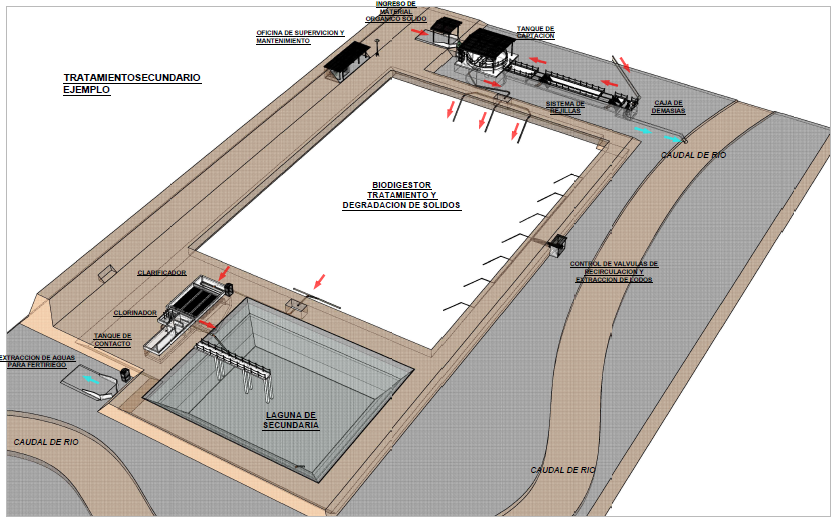
\includegraphics[width=1\linewidth]{images/201901-gfong-imagen08} 

}

\caption{Modelo Planta de tratamiento desechos sólidos y aguas residuales}\label{fig:unnamed-chunk-24}
\end{figure}

\begin{figure}[H]

{\centering 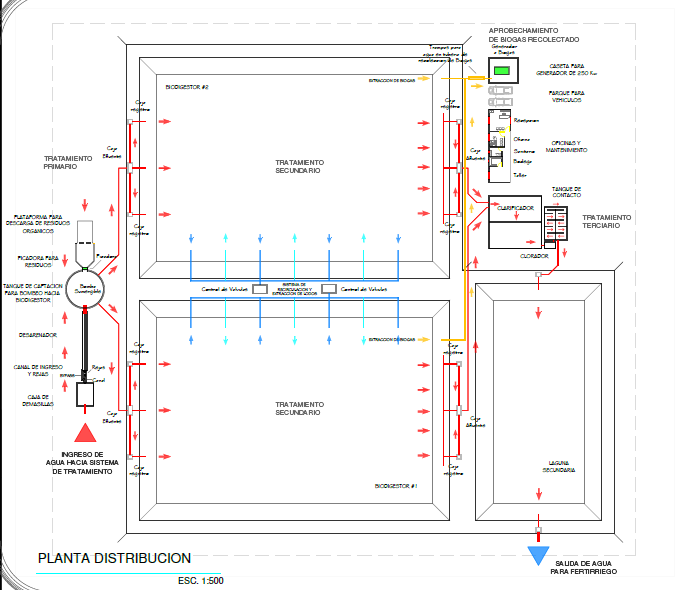
\includegraphics[width=1\linewidth]{images/201901-gfong-imagen09} 

}

\caption{Vista Planta de tratamiento desechos sólidos y aguas residuales}\label{fig:unnamed-chunk-25}
\end{figure}

\hypertarget{lcalmo}{%
\chapter{Diseño y plan de mantenimiento de una línea de embotellado de agua de coco para la empresa Comeragua S.A. / Gordian®}\label{lcalmo}}

\begin {flushleft}

\begin{tcolorbox}[sharp corners=uphill, colback=fondo, colframe=fondo, arc=6mm, boxrule=0mm, boxsep=2mm,  opacityframe=0.19,  opacityback=0.19]

\begin{minipage}[c]{3cm}

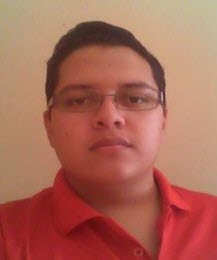
\includegraphics[width=2.5cm,height=\textheight]{images/201901-lcalmo-photo.jpg}

\end{minipage}\begin{minipage}[c]{12cm}

\textbf{Autor:} \emph{Luis Alberto Calmo Galindo}\\
\textbf{Correo electrónico:} \emph{\href{mailto:calmogear@gmail.com}{\nolinkurl{calmogear@gmail.com}}}\\
\textbf{Fecha:} \emph{04 de abril de 2019}

\end{minipage}

\end {tcolorbox}

\end {flushleft}

\hypertarget{resumen-2}{%
\section*{Resumen}\label{resumen-2}}
\addcontentsline{toc}{section}{Resumen}

Un proyecto de EPS normalmente consta de tres fases: la primera de ellas consiste en realizar una investigación interna sobre el uso del agua y cómo hacer más eficiente su consume; esto con el objetivo de ayudar al medio ambiente y así mismo reducir los costos de funcionamiento de las bombas y equipos de distribución. La segunda fase es básicamente el desarrollo del proyecto de EPS, el objetivo principal fue desarrollar el diseño de una línea de embotellado de agua de coco libre de preservantes artificiales, utilizando equipos presentes en la planta y complementando con otros adicionales; también se creó un plan de mantenimiento preventivo -- corrective, clasificando a los equipos con base en su criticidad. Por último la etapa de docencia, en donde se impartieron capacitaciones al personal del área de mantenimiento, siendo la primera ``El procedimiento correcto del mantenimiento'' utilizando las normativas internas de Gordian® y la segunda fue la ``implementación del programa 5S''.

\hypertarget{abstract-2}{%
\section*{Abstract}\label{abstract-2}}
\addcontentsline{toc}{section}{Abstract}

An EPS project usually consists of three phases: the first one consisted in carrying out an internal investigation on the use of water and how to make its consumption more efficient, this with the aim of helping the environment and also reduce operating costs of pumps and distribution equipment. The second phase is basically the development of the EPS project, the main objective was to develop the design of a coconut water bottling line free of artificial preservatives, using equipment present in the plant and complementing with additional ones; a preventive-corrective maintenance plan was also created, classifying the equipment according to their criticality. Finally, the teaching stage, where training was given to maintenance personnel, the first training being ``the correct maintenance procedure'' using Gordian® internal regulations, and the second was the ``implementation of the 5S program''.

\hypertarget{palabras-clave-2}{%
\section*{Palabras Clave:}\label{palabras-clave-2}}
\addcontentsline{toc}{section}{Palabras Clave:}

\emph{Agua de coco, línea de embotellado, diseño, plan de mantenimiento, criticidad.}

\begin {multicols}{2}

\hypertarget{introduccion-3}{%
\section{Introducción}\label{introduccion-3}}

Las bebidas embotelladas son consumidas en la mayoría de los países debido a su facilidad de distribución, almacenaje y transporte. Hay diferentes tipos de bebidas, dentro de las cuales se podrían clasificar en naturales y artificiales; las naturales son extraídas directamente de los frutos o vegetales y sin mayor modificación en el sabor; en cambio las artificiales, normalmente cuentan con colorantes, saborizantes, entre otros aditivos que modifican el sabor y otras propiedades de las bebidas.

Tomando en cuenta lo anteriormente planteado, la empresa Comeragua S.A./Gordian®, ha planteado implementar una línea de embotellado de agua de coco 100 \% natural y libre de preservantes y aditivos. Por lo que fue necesario desarrollar un diseño completo de la línea de producción, como también un plan de mantenimiento de tipo preventivo -- correctivo.

\hypertarget{articulo-2}{%
\section{Artículo}\label{articulo-2}}

Desde un principio la planta Gordian® se ha dedicado a comercializar aguacate Hass, así como también a producir guacamole, utilizando ingredientes frescos y 100\% naturales. Los productos están libres de conservantes artificiales, ya que la empresa cuenta con la más alta tecnología de pasteurización en frío; esta tecnología es conocida como HPP (High Pressure Processing).

\medskip

Ya que su materia prima base es el aguacate Hass se suelen tener dificultades de producción en temporadas en las que este aguacate no está disponible; específicamene debido a factores climatológicos o bien por el mismo ciclo de cosecha del fruto. Tomando esto en cuenta en Gordian® ha surgido la iniciativa de implementar un nuevo producto que no tenga dependencia del aguacate Hass; una de las ideas más sobresalientes ha sido la de embotellar agua de coco.

\hypertarget{el-agua-de-coco}{%
\subsection{El agua de coco}\label{el-agua-de-coco}}

El agua de coco es incolora, de aspecto claro y ligeramente dulce; dentro de la nuez es estéril, lo que significa que está libre de microorganismos. Siempre que se expone al aire o al ambiente externo, el producto está expuesto a la contaminación microbiológica y a su deterioro. La manipulación apropiada y el control de la temperatura, desde el momento de la recolección y durante el proceso de la cadena, son esenciales para que el agua de coco pueda conservar las cualidades inherentes que tenía antes del proceso. La cantidad de agua que se puede extraer de un coco depende de la variedad y el estado de maduración del mismo.

Tiene propiedades isotónicas; esto hace que sea muy recomendable para tratamientos de rehidratación en caso de enfermedades como el dengue y la chikungunya. Como anteriormente fue mencionado, el agua de coco debe tener un sabor agradable sin trazas amargas o mal sabor. No se debe consumir agua de coco que ha estado fuera de la nuez por demasiado tiempo sin refrigeración, debido a que es un product que con facilidad puede ser contaminado por gérmenes y bacterias en ambientes poco controlados.

\bigskip

\begin {flushleft}
\noindent\begin{minipage}[c]{\columnwidth}


\includegraphics[width=1\linewidth]{images/201901-lcalmo-imagen01}
\figcaption{La mejor bebida isotónica del mundo: el agua de coco}

\end{minipage}

\end {flushleft}

\medskip

\hypertarget{embotellado-de-bebidas}{%
\subsection{Embotellado de bebidas}\label{embotellado-de-bebidas}}

Un proceso de embotellado conlleva una serie de distintos pasos o etapas en donde se busca hacer más eficiente el uso de la materia prima; dependiendo de la complejidad del proceso así va a ser la cantidad de equipos y maquinaria necesarios para el embotellado. Se puede decir que cada proceso depende mucho de la bebida que se pretende embotellar; además, hay que tomar en cuenta el tipo de envase a utilizar, la velocidad de producción, entre otros factores.

\medskip

De manera general el embotellado se inicia con el tratamiento de la bebida, bien sea en su preparación o extracción; a continuación se procede a preparar los envases y por consiguiente se introduce la bebida a los envases normalmente de forma automatizada. Las bebidas son pasteurizadas o filtradas de manera que sean seguras para el consumo; es importante enfatizar que la pasteurización extiende la vida anaquel después de ser embotellada.

\end {multicols}

\begin{center}\rule{0.5\linewidth}{\linethickness}\end{center}

\begin{figure}[H]

{\centering 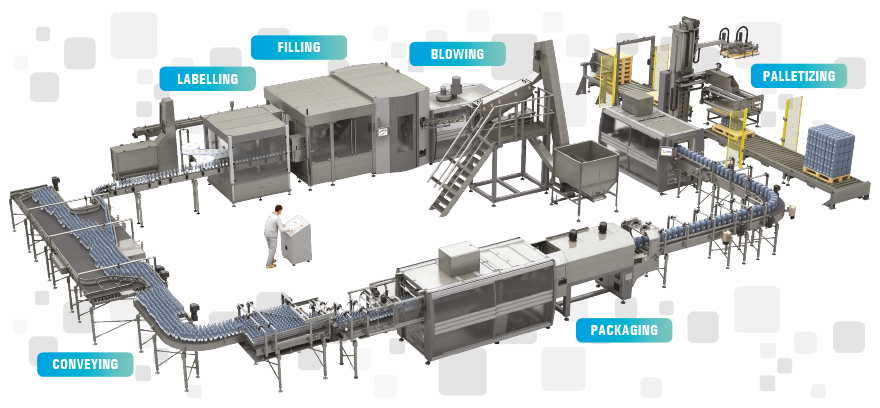
\includegraphics[width=1\linewidth]{images/201901-lcalmo-imagen02} 

}

\caption{Líneas completas de embotellado y embalaje}\label{fig:unnamed-chunk-28}
\end{figure}

\begin {multicols}{2}

\hypertarget{linea-de-embotellado-de-agua-de-coco}{%
\subsection{Línea de embotellado de agua de coco}\label{linea-de-embotellado-de-agua-de-coco}}

El diseño de la línea de embotellado se hizo con base en algunos equipos ya presentes en la planta de Gordian®, con los cuales se tenía que buscar una armonía para que la línea funcionara de acuerdo con sus especificaciones y requerimientos.

Básicamente la línea se dividía en tres secciones o etapas: la primera es la del ``manejo del coco'', en donde es lavado y sanitizado antes de extraer la bebida; esta etapa es importante ya que para conseguir una alta calidad e inocuidad es necesario que el fruto entre completamente limpio a la máquina cortadora; la segunda fase es la del ``tratamiento del agua de coco'', con el fin de recolectar, filtrar y mantener a una baja temperatura el producto, ya que esto evita una descomposición prematura del agua; por ultimo, se procede al área de embotellado; en esta etapa se preparan y llenan los envases con el product; también se hace el empaquetado y entarimado.

Cabe destacar que además de la filtración del agua de coco también se cuenta con un sistema de HPP, el cual permite una alta inocuidad, logrando con esto un producto apto y de calidad para el consumo humano.

\hypertarget{plan-de-mantenimiento}{%
\subsection{Plan de mantenimiento}\label{plan-de-mantenimiento}}

Dependiendo del tipo de mantenimiento asignado a una máquina así va a ser su funcionamiento y durabilidad; generalmente se puede clasificar en correctivo, preventivo y predictivo. Existen otras clasificaciones del mantenimiento, pero estas tres son las principales y a las que comúnmente se puede tener acceso. El mantenimiento incluido en este plan se centraliza en el tipo preventivo y correctivo; se excluye cualquier otro tipo como el predictivo porque se necesitaría una gran inversión y los equipos no son de la categoría adecuada para este tipo de mantenimiento.

La criticidad es la importancia asignada a una máquina o equipo respecto del efecto que puede ocasionar una falla o avería en un proceso determinado, cada equipo tiene que ser evaluado de acuerdo con márgenes que son importantes para la producción. La criticidad puede ser evaluada con diferentes referencias, por ejemplo, la inocuidad, calidad, seguridad, materia prima usada, consumo de energía, desgaste, vibración, entre otras.

El plan de mantenimiento desarrollado tomará en cuenta la inocuidad, calidad y seguridad del personal, ya que estos tres aspectos son de gran importancia para el proceso de embotellado de agua de coco. Es de esperarse que haya equipos con diferentes aspectos a tomar en cuenta como el desgaste, pero esto será compensado asignando una verificación más minuciosa respecto de los demás.

\end {multicols}

\begin{center}\rule{0.5\linewidth}{\linethickness}\end{center}

\begin{figure}[H]

{\centering 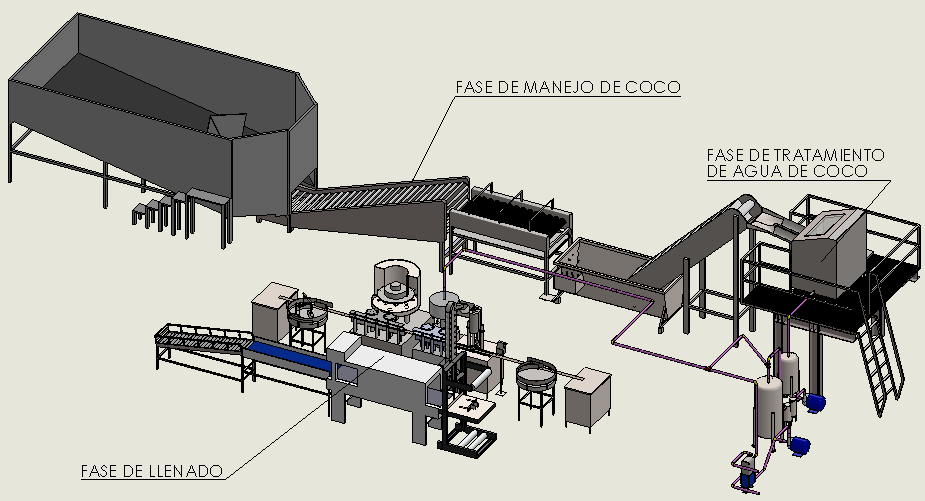
\includegraphics[width=1\linewidth]{images/201901-lcalmo-imagen03} 

}

\caption{Diseño y plan de mantenimiento de una línea de embotellado de agua de coco para la empresa Comeragua S.A. / Gordian®}\label{fig:unnamed-chunk-29}
\end{figure}

\begin {multicols}{2}

\bigskip

\hypertarget{conclusiones-2}{%
\section{Conclusiones}\label{conclusiones-2}}

\begin{itemize}
\item
  Hay distintos equipos disponibles para el embotellado de bebidas, en este proyecto se han propuesto los más adecuados para el proceso de embotellado de agua de coco.
\item
  Las máquinas con mayor criticidad son sin lugar a dudas las que se encuentran en contacto continuo con el agua de coco, ya que de acuerdo con el método de criticidad establecido en este document, los factores principales son la inocuidad, calidad y seguridad de los empleados.
\item
  El plan de mantenimiento generado de tipo preventivo y correctivo es adecuado al tipo de máquinas y equipos incluidos, puesto que un mantenimiento más complejo aumentaría los costos innecesariamente, así también, posteriormente, será necesario contar con un stock de repuestos acorde a la criticidad establecida en el plan.
\end{itemize}

\hypertarget{referencias-2}{%
\section{Referencias}\label{referencias-2}}

\begin{itemize}
\item
  CALMO GALINDO, Luis Alberto. (2017). \emph{Diseño y plan de mantenimiento de una línea de embotellado de agua de coco para la empresa Comeragua S.A. / Gordian®.} Trabajo de graduación de Ing. Mecánica. Facultad de Ingeniería, Universidad de San Carlos de Guatemala\footnote{\url{http://biblioteca.usac.edu.gt/tesis/08/08_0963_M.pdf}}.*
\item
  DÍAZ NAVARRO, Juan. \emph{Técnicas de mantenimiento industrial.} 2a ed.~Revisada. Cádiz, 2010. 318 p.~ISBN: 9788461377473.
\item
  MUÑOZ ABELLA, Belén. \emph{Mantenimiento Industrial.} Madrid. Material de curso Tecnología de Máquinas. Ingeniería Industrial. Facultad de Ingeniería. Universidad Carlos III de Madrid, 2003\footnote{\url{http://ocw.uc3m.es/ingenieria-mecanica/tecnologia-de-maquinas/material-de-clase-1/MANTENIMIENTO.pdf}}. {[}Consulta en línea: Octubre de 2015{]}.
\item
  PYTEL, Andrew y SINGER, Ferdinad. \emph{Resistencia de materiales.} Traducción de la 4a ed.~México: Alfaomega 2008. 584 p.~ISBN: 9789701510568 y 9701510569.
\item
  ROLLE, Rosa. \emph{Buenas prácticas para la producción en pequeña escala de agua de coco embotellada.} FAO, Roma, 2007. 49 p\footnote{\url{ftp://ftp.fao.org/docrep/fao/010/a1418s/a1418s.pdf}}. {[}Consulta en línea: Septiembre de 2015{]}.
\item
  SISTEMAS HIDRONEUMÁTICOS C.A. \emph{Manual de procedimiento para el cálculo y selección de sistemas de bombeo.} Caracas, 76 p\footnote{\url{http://www.sishica.com/sishica/download/Manual.pdf}}. {[}Consulta en línea: Octubre de 2015{]}.
\item
  TORRES RIVERA, Cesar Alberto. \emph{Diseño de un sistema de limpieza en el sitio de tipo sanitario (CIP) para una línea de llenado en un salón de embotellado en la industria de cerveza.} Trabajo de graduación de Ing. Mecánica Industrial. Facultad de Ingeniería, Universidad de San Carlos de Guatemala, 2012. 174 p.
\end{itemize}

\end {multicols}

\hypertarget{rherrera}{%
\chapter{Optimización de procesos a través de un EPS}\label{rherrera}}

\begin {flushleft}

\begin{tcolorbox}[sharp corners=uphill, colback=fondo, colframe=fondo, arc=6mm, boxrule=0mm, boxsep=2mm,  opacityframe=0.19,  opacityback=0.19]

\begin{minipage}[c]{3cm}

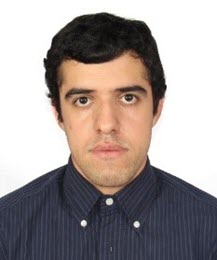
\includegraphics[width=2.5cm,height=\textheight]{images/201901-rherrera-photo.jpg}

\end{minipage}\begin{minipage}[c]{12cm}

\textbf{Autor:} \emph{Rodrigo Antonio Herrera de León}\\
\textbf{Correo electrónico:} \emph{\href{mailto:herrerarodrigo750@gmail.com}{\nolinkurl{herrerarodrigo750@gmail.com}}}\\
\textbf{Fecha:} \emph{27 de marzo de 2019}

\end{minipage}

\end {tcolorbox}

\end {flushleft}

\hypertarget{resumen-3}{%
\section*{Resumen}\label{resumen-3}}
\addcontentsline{toc}{section}{Resumen}

La Facultad de Humanidades de la Universidad de San Carlos de Guatemala busca la automatización de sus procesos administrativos, ya que la ejecución manual consume una gran cantidad de recursos e incrementa la probabilidad de error humano. El presente artículo trata sobre la automatización del proceso de recuperaciones. Este incluye la habilitación del pago de recuperaciones en el sistema de información financiera de la universidad, la asignación a recuperaciones, su pago por parte de los estudiantes y el ingreso de notas por parte de los catedráticos. Dicho proceso, antes ejecutado de forma manual, fue automatizado al ampliar las funcionalidades del portal web previamente existente, lo que permite su ejecución en línea y aprovecha los recursos tecnológicos disponibles. La respuesta ante los resultados del proyecto fue positiva por parte de la comunidad estudiantil, de los catedráticos y del personal de la Facultad; se cumplió con las expectativas de quienes propusieron el proyecto y de quienes lo desarrollaron e implementaron.

\hypertarget{abstract-3}{%
\section*{Abstract}\label{abstract-3}}
\addcontentsline{toc}{section}{Abstract}

The Faculty of Humanities of the University of San Carlos of Guatemala seeks to automate its administrative processes because manual execution consumes a large amount of resources and increases the probability of human errors. The present article is about the automation of the recovery process. This includes the enabling of recoveries' payment in the finance information system of the university, the assignment to recoveries, its payment by the students, and the entry of notes by the teachers. This process, previously executed manually, was automated by extending the functionality of the already existing web portal, which allows its execution online and takes advantage of the available technological resources. The response to the results of the project was positive, from the student community and teachers and the Faculty staff; it was fulfilled with the expectations of those who proposed the project and of those who developed and implemented it.

\hypertarget{palabras-clave-3}{%
\section*{Palabras Clave:}\label{palabras-clave-3}}
\addcontentsline{toc}{section}{Palabras Clave:}

\emph{Optimización, automatización, EPS, USAC.}

\begin {multicols}{2}

\hypertarget{introduccion-4}{%
\section{Introducción}\label{introduccion-4}}

Actualmente, en varias organizaciones e instituciones, se busca automatizar los procesos a través de la transformación de tareas ejecutadas manualmente, y las realizadas en forma parcial o totalmente por computadora. Esto no solo optimiza el uso de los recursos, sino también reduce la posibilidad de error humano. La oficina de Control Académico de la Facultad de Humanidades de la Universidad de San Carlos de Guatemala tiene a su cargo la gestión de los estudiantes de todas las carreras de la Facultad. Dicha gestión implica la ejecución de muchos procesos administrativos necesarios para atender la gran cantidad de estudiantes. Por esta razón la Facultad de Humanidades ya ha automatizado varios de sus procesos para atender eficientemente a los estudiantes actualmente inscritos.

Gran parte de esta automatización se ha realizado con el portal web de la Facultad al que tienen acceso los estudiantes y catedráticos. Uno de los procesos automatizados es el de asignación a exámenes de retrasada o recuperaciones. Este último se desarrolló como proyecto de Ejercicio Profesional Supervisado (EPS), cuya implementación y resultados serán mostrados en el presente artículo.

\hypertarget{articulo-3}{%
\section{Artículo}\label{articulo-3}}

\hypertarget{problema}{%
\subsection{Problema}\label{problema}}

Antes de la implementación del proyecto, la asignación y pago de recuperaciones se ejecutaba de forma manual, lo cual, debido a la gran cantidad de estudiantes, consumía demasiados recursos. El flujo era el siguiente:

\begin{itemize}
\item
  El Departamento de Control Académico realizaba manualmente la habilitación del pago de las recuperaciones en el SIIF (Sistema Integrado de Información Financiera). De esta manera, se elegían uno por uno los cursos que iban a estar disponibles para que el estudiante pagara por sus recuperaciones. Este proceso duraba aproximadamente cuatro horas.
\item
  El estudiante se presentaba el día de la recuperación y entregaba al catedrático el comprobante de pago junto con su examen.
\item
  El estudiante se presentaba el día de la recuperación y entregaba al catedrático, junto con su examen, el comprobante de pago como constancia de pago de su examen.
\item
  El catedrático calificaba los exámenes e ingresaba las notas (zona y recuperación) en archivo con formato XLS.
\item
  El catedrático entregaba su archivo con las notas a Control Académico durante la semana calendarizada. Este último, al recibirlo, tenía que verificar manualmente que todos los estudiantes examinados tuvieran derecho a examen.
\item
  Una vez terminado el período de recepción de notas, Control Académico, junto con la Unidad de Sistemas, ingresaban las notas. Este proceso duraba generalmente cinco días hábiles.
\item
  El estudiante podía ver sus notas el día posterior a la finalización del ingreso de estas.
\item
  Control Académico verificaba que todo estuviera correctamente procesado. Este proceso duraba generalmente 5 días hábiles.
\end{itemize}

\hypertarget{solucion-planteada}{%
\subsection{Solución planteada}\label{solucion-planteada}}

Con base en las necesidades planteadas se establecieron los siguientes objetivos para el proyecto:

\begin{itemize}
\item
  Agilizar la habilitación del pago de recuperaciones en el SIIF.
\item
  Permitir a los catedráticos el ingreso de notas de recuperación a través del portal web de la Facultad, asegurando que su valor fuera válido y sin necesitar ingresar la zona.
\item
  Automatizar los filtros de asignaciones a las recuperaciones y la confirmación de los pagos correspondientes.
\item
  Permitir a los catedráticos el ingreso de notas de recuperación a través del portal web de la Facultad, asegurando que su valor sea válido y sin necesitar ingresar la zona.
\end{itemize}

\hypertarget{desarrollo-e-implementacion-del-proyecto}{%
\subsection{Desarrollo e implementación del proyecto}\label{desarrollo-e-implementacion-del-proyecto}}

El proyecto se integró al sistema de la Facultad, ampliando las funcionalidades de cada usuario; las tareas se ejecutan ahora de manera más rápida que cuando se hacían manualmente y se lleva un registro de todas las acciones realizadas.

Para automatizar la confirmación de los pagos, se desarrolló un servicio web que permite manejar la comunicación con el SIIF. De esta forma, en el momento que el banco notifique el pago de una recuperación al SIIF, este le informará al sistema de la Facultad para confirmar la asignación del estudiante.

\end {multicols}

\begin{center}\rule{0.5\linewidth}{\linethickness}\end{center}

\begin{figure}[H]

{\centering 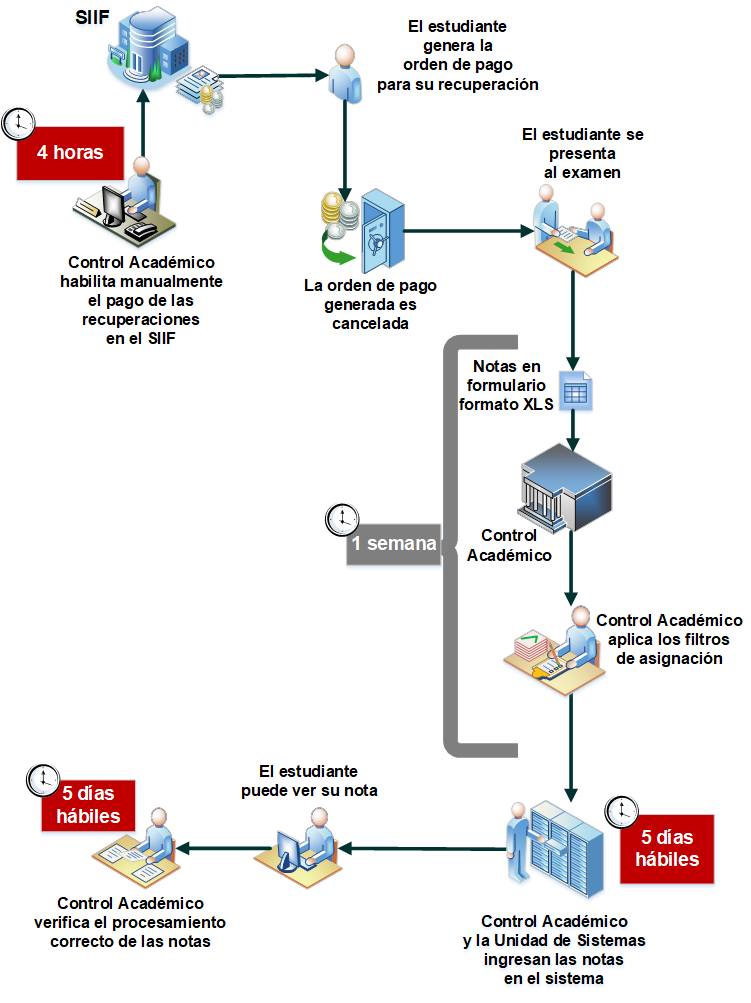
\includegraphics[width=0.75\linewidth]{images/201901-rherrera-imagen01} 

}

\caption{Proceso actual del problema presentado }\label{fig:unnamed-chunk-30}
\end{figure}

\begin {multicols}{2}

\hypertarget{proyecto-implementado}{%
\subsection{Proyecto implementado}\label{proyecto-implementado}}

Una vez implementado el proyecto, el flujo del proceso cambió de la siguiente manera:

\begin{itemize}
\item
  La habilitación del pago de recuperaciones en el SIIF se realiza con ayuda del portal web. Este proceso dura aproximadamente cinco minutos.
\item
  El estudiante ingresa con su usuario al portal de la Facultad y genera la orden de pago para la recuperación que desea. Se filtran las opciones, de manera que solo aparecerán disponibles las recuperaciones a las que el estudiante tenga derecho.
\item
  El estudiante cancela la orden de pago generada. Al hacerlo, el banco, por medio del SIIF, notificará al sistema de la Facultad los datos de la recuperación que ha sido pagada. Al recibir dicha información, se confirma la asignación del estudiante a la recuperación respectiva.
\item
  El estudiante se presenta al examen, sin tener que entregar la constancia de pago.
\item
  El catedrático ingresa las notas de recuperación, con su usuario, al portal de la Facultad. El portal verifica que el valor de las notas ingresadas esté en el rango válido y lo asocia a la nota de la zona respectiva almacenada en el sistema.
\item
  Las notas podrán ser vistas por el estudiante a partir del día siguiente del que fueron cargadas.
\end{itemize}

\end {multicols}

\begin{center}\rule{0.5\linewidth}{\linethickness}\end{center}

\begin{figure}[H]

{\centering 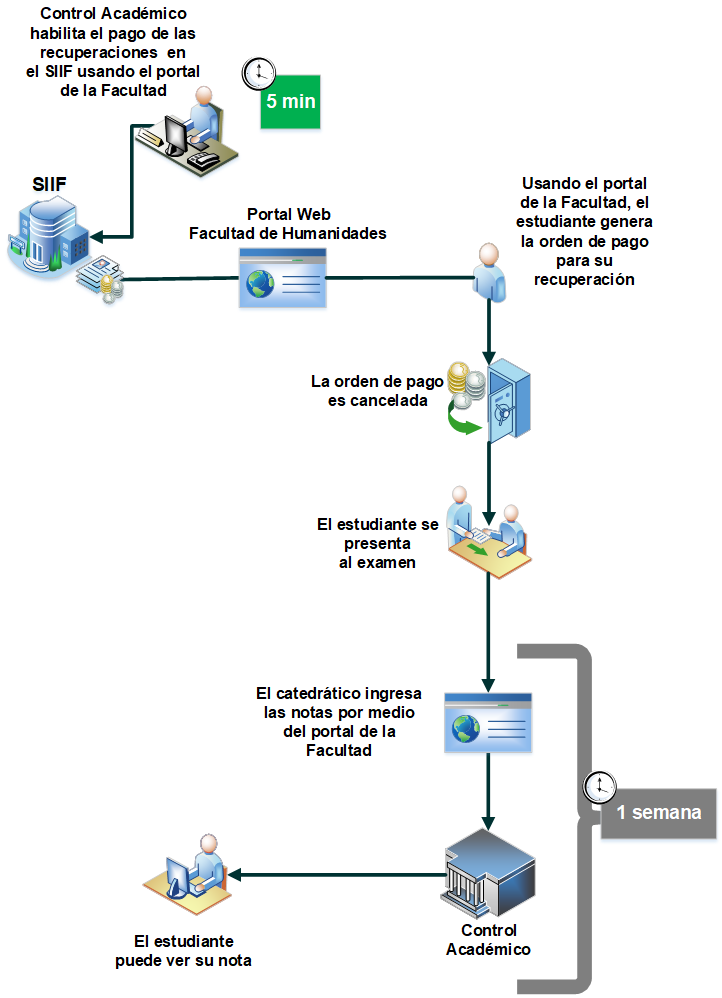
\includegraphics[width=0.6\linewidth]{images/201901-rherrera-imagen02} 

}

\caption{Mejoramiento de proceso de pago de recuperaciones}\label{fig:unnamed-chunk-31}
\end{figure}

\begin {multicols}{2}

\hypertarget{conclusiones-3}{%
\section{Conclusiones}\label{conclusiones-3}}

\begin{itemize}
\item
  La automatización del módulo de recuperación es un gran avance para la Facultad de Humanidades, en su proyección respecto del uso las tecnologías de actualidad para resolver sus necesidades.
\item
  La nueva forma de habilitar el pago de las recuperaciones en el SIIF es aproximadamente 80 \% más rápida que la forma anterior.
\item
  La asignación y generación de las órdenes de pago de recuperación por medio de una herramienta web permite tener un mayor control y orden en dichos procesos, y brindar un mejor servicio a los estudiantes.
\item
  La automatización de los filtros de asignación a recuperaciones y la confirmación de pagos de estas permiten su ejecución casi inmediata y remueven carga de trabajo al personal de la Facultad.
\item
  El ingreso de notas por medio de una herramienta web mejora la integridad de este proceso, ya que reduce la información que el catedrático tiene que ingresar y verifica que las notas estén en un rango valido.
\item
  El sistema actual permite que los estudiantes puedan ver su nota de recuperación mucho antes de lo que lo permitía el sistema anterior.
\end{itemize}

\hypertarget{referencias-3}{%
\section{Referencias}\label{referencias-3}}

\begin{itemize}
\tightlist
\item
  HERRERA DE LEÓN, Rodrigo Antonio. (2017). \emph{Automatización del módulo de recuperación en la oficina de Control Académico, Facultad de Humanidades, Universidad de San Carlos de Guatemala\footnote{\url{http://www.repositorio.usac.edu.gt/8239/1/Rodrigo} Antonio Herrera De León.pdf}.} {[}Consulta en línea: 2019{]}.
\end{itemize}

\end {multicols}

\hypertarget{cchicojay}{%
\chapter{Programa Facebook Live y su aplicación en el campo de la docencia}\label{cchicojay}}

\begin {flushleft}

\begin{tcolorbox}[sharp corners=uphill, colback=fondo, colframe=fondo, arc=6mm, boxrule=0mm, boxsep=2mm,  opacityframe=0.19,  opacityback=0.19]

\begin{minipage}[c]{3cm}

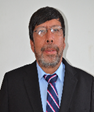
\includegraphics[width=2.5cm,height=\textheight]{images/201901-cchicojay-photo.png}

\end{minipage}\begin{minipage}[c]{12cm}

\textbf{Autor:} \emph{Carlos Aníbal Chicojay Coloma}\\
\textbf{Correo electrónico:} \emph{\href{mailto:anibalchicojay@yahoo.com}{\nolinkurl{anibalchicojay@yahoo.com}}}\\
\textbf{Fecha:} \emph{27 de marzo de 2019}

\end{minipage}

\end {tcolorbox}

\end {flushleft}

\hypertarget{resumen-4}{%
\section*{Resumen}\label{resumen-4}}
\addcontentsline{toc}{section}{Resumen}

Dada la convergencia digital y tecnológica, los Espacios Virtuales de Aprendizaje (EVA) cada vez son más aceptados por los estudiantes de la Universidad de San Carlos de Guatemala. La mayor parte de plataformas de los EVA incluyen intercambio de material digital, pero es necesario tener una comunicación en tiempo real con el estudiante. La plataforma Facebook, incluye la opción de transmisiones en vivo, con la opción de compartir pantalla; esto facilita impartir una clase online utilizando Power Point, PDF, Word, entre otros. Para mejor desempeño se recomienda abrir una Fan Page y desde allí correr la opción de ``Transmitir en vivo'' y luego compartir pantalla; de esta forma el profesor puede recibir las preguntas escritas de los estudiantes y responder ya sea por el mismo chat, o por voz. Ventajas: 1) No se debe de instalar nada adicional en el computador, 2) Para propósitos docentes no existe límite de participantes, 3) La clase queda grabada para poderla ver posteriormente; 4) El estudiante puede seguir la transmisión desde cualquier dispositivo móvil. 5) No depende del servidor de la Universidad. Desventajas: 1) Se necesita conexión estable a internet; si la señal es inestable, el botón ``Transmitir en vivo'' aparecerá deshabilitado. 2) Por el momento, no es posible alternar entre la cámara y pantalla, ni transmitir una película sin instalar software adicional al computador, aunque si presenta la opción de subir videos. Se realizó a manera de ensayo una prueba con la última parte del curso Instrumentación Mecánica en la Escuela de Ingeniería Mecánica; el estudiante valoró la opción de tener acceso a las clases en diferido y las veces que se quisieran.

\hypertarget{abstract-4}{%
\section*{Abstract}\label{abstract-4}}
\addcontentsline{toc}{section}{Abstract}

Given the digital and technological convergence, virtual learning spaces (LVS) are increasingly accepted by students of the University of San Carlos de Guatemala. Most platforms of the LVS, include exchange of digital material, but it is necessary to have a real-time communication with the student. The Facebook platform includes the option of live broadcasts, with the option of screen sharing, facilitating an online class using Power Point, PDF, Word, and others. For a better performance, it is recommended to open a Fan Page and from it run the option of ``Transmit live'' and then share the screen, in this way the teacher can receive written questions from the students and respond either by the same chat, or by voice. Advantages: 1) No additional installation should be installed in the computer, 2) For teaching purposes there is no limit of participants, 3) The class is recorded for later viewing, 4) The student can follow the transmission from any mobile device. 5) It does not depend on the server of the University. Disadvantages: 1) A stable internet connection is needed, if the signal is unstable, the ``Transmit live'' button will be disabled. 2) At the moment, it is not possible to alternate between the camera and the screen, nor to transmit a movie without installing additional software to the computer, although it does present the option of uploading videos. A test with the last part of the Mechanical Instrumentation course at the School of Mechanical Engineering; the student valued the option of having access to the classes in deferred and the times that they wanted.

\hypertarget{palabras-clave-4}{%
\section*{Palabras Clave:}\label{palabras-clave-4}}
\addcontentsline{toc}{section}{Palabras Clave:}

\emph{Facebook Live, Enseñanza, Uso de las TIC.}

\begin {multicols}{2}

\hypertarget{introduccion-5}{%
\section{Introducción}\label{introduccion-5}}

El avance tecnológico en el área digital ha aparecido en varios campos del conocimiento, las tecnologías de la información y comunicación, en principio, y ahora el internet de las cosas depara un futuro que no imaginábamos y el campo de la educación no escapa a ello. Gran parte de esto es consecuencia de la tecnología que poco a poco se ha ido abriendo paso en el sector de la educación, hasta tal punto que ahora se puede hablar de una rama de la tecnología que únicamente se centra en la educación. Las innovaciones tecnológicas permiten que los estudiantes del presente disfruten de muchas experiencias y alternativas que antaño no podían ni siquiera concebirse. La educación a través de la red experimentó un notable crecimiento a mediados de la primera década del siglo XXI. Hoy en día, en algunos casos ya se habla de una supremacía del canal online de cara a la transmisión de determinados tipos de conocimiento, particularmente aquellos sujetos a una interacción intensa profesor-alumno y con los alumnos entre sí. {[}1{]} Aunque la adaptación de estas nuevas tecnologías no ocurre a la velocidad con la que estas aparecen. Dentro de esto no se debe dejar al margen el auge que han tenido los Smartphones, que tienen como aliadas a las TIC, las cuales pueden ser de gran utilizdad en educación. Por esta razón, la UNESCO cree más efectivo regular el empleo de la telefonía móvil con fines pedagógicos. {[}1{]}

\hypertarget{articulo-4}{%
\section{Artículo}\label{articulo-4}}

\hypertarget{antecedentes}{%
\subsection{Antecedentes}\label{antecedentes}}

Cada vez son más utilizados los Espacios Virtuales de Aprendizaje. La educación a distancia cada vez es más aceptada por el estudiante por las ventajas que esta presenta. En la Escuela de Ingeniería Mecánica de la Universidad de San Carlos de Guatemala, la plataforma Moodle es la que oficialmente ofrece la Facultad de Ingeniería, la cual es utilizada por un número limitado de profesores. Dicha plataforma aplica para el intercambio de material en ambas vías, pero no presenta la función de audio y video en tiempo real.

\hypertarget{la-web-2.0}{%
\subsection{La Web 2.0}\label{la-web-2.0}}

Es una segunda generación de servicios basados en la web; esta enfatiza en la colaboración online, la conectividad y posibilidad de compartir contenidos entre los usuarios. Implica la evolución de las aplicaciones digitales hacía aplicaciones dirigidas al usuario final, que incluyen servicios como redes sociales, blogs, wikis, entre y otros {[}2{]}.

\hypertarget{las-redes-sociales}{%
\subsection{Las redes sociales}\label{las-redes-sociales}}

En los últimos años, el nacimiento y desarrollo de estos medios ha sufrido un crecimiento estratosférico, convirtiéndose en parte fundamental y cotidiana de nuestras vidas. Lo habitual es que la mayoría de los internautas cuente con más de un perfil social. {[}3{]} En la actualidad, entre todas las redes sociales, Facebookresulta ser la red de más uso a nivel mundial {[}4{]}.

\hypertarget{objetivos-1}{%
\section{Objetivos}\label{objetivos-1}}

Presentar la forma de operar la plataforma Facebook en el proceso educativo, potencializando el uso de la opción de transmisiones en vivo, compartiendo la pantalla del computador.

Analizar la eficiencia y aceptación de la aplicación, derivado de un ensayo realizado en el curso de Instrumentación Mecánica, del pénsum de estudios de la Carrera de Ingeniería Mecánica, de la Universidad de San Carlos de Guatemala.

\hypertarget{facebook-dentro-de-un-espacio-virtual-de-aprendizaje}{%
\section{Facebook dentro de un espacio virtual de aprendizaje}\label{facebook-dentro-de-un-espacio-virtual-de-aprendizaje}}

La aplicación de Facebook dentro de un EVA, puede significar un complemento a las plataformas tradicionales como Moodle, que son bastante utilizadas; en ella es posible interactuar entre profesor y estudiante; sus funciones se resumen en envió de material en ambas direcciones, profesor estudiante, estudiante profesor, foros, y chats.

\hypertarget{streaming}{%
\subsection{Streaming}\label{streaming}}

Las emisiones en streaming han sido una de las tendencias de marketing actuales, ya que cada vez aparecen más aplicaciones que permiten hacerlas, y más usuarios aprovechándose de este servicio tan requerido para llegar a las masas en vivo. El streaming permite escuchar música o ver vídeos sin tener que descargarlos previamente. Antes de que apareciera esta tecnología era necesario descargar por completo el archivo para reproducirlo. Normalmente estos ficheros son muy pesados, pero con dicha tecnología, al no tener que descargarlos completamente, la transmisión y reproducción pueden realizarse casi simultáneamente, ya que descargan pequeños paquetes fragmentados. Esto ha sido posible gracias a los avances tecnológicos y a la generalización del uso de la banda ancha, indispensable para que la emisión sea continua, sin cortes y de calidad. {[}5{]}

\hypertarget{facebook-live}{%
\subsection{Facebook Live}\label{facebook-live}}

Es la nueva herramienta que ha introducido Facebook para la emisión de vídeos en directo desde el computador y dispositivos móviles, la cual fue apareciendo paulatinamente alrededor del mundo a partir del año 2017. Para el mundo de la educación, esta plataforma incluye una gran herramienta: ``Share Scrren'', en la cual se puede compartir todo lo que sucede en la pantalla del computador mientras el profesor explica el contenido. El estudiante en tiempo real recibe audio y video en cualquier dispositivo conectado a internet que posea la aplicación Facebook instalada. Además, presenta la ventaja que el sistema graba la actividad para que el estudiante, en cualquier momento posterior pueda entrar a verla en diferido; se puede utilizar un chat, en el cual el estudiante realiza sus consultas en tiempo real, o en diferido. En este último caso, el profesor debe de entrar posteriormente al programa para contestar las consultas realizadas posteriormente a la transmisión en vivo.

\hypertarget{procedimiento-para-efectuar-trasmision-de-clase-en-vivo-por-facebook-live}{%
\section{Procedimiento para efectuar trasmisión de clase en vivo por Facebook Live}\label{procedimiento-para-efectuar-trasmision-de-clase-en-vivo-por-facebook-live}}

El procedimiento acá presentado se lleva a cabo sin instalar nada adicional al computador. Los pasos a seguir en la configuración para la transmisión son los siguientes:

\begin{enumerate}
\def\labelenumi{\alph{enumi}.}
\item
  Si aún no se posee, abrir una cuenta en Facebook: \url{https://www.facebook.com/}
\item
  Crear una página, o fan page, para uso exclusivo de las transmisiones en vivo
\item
  Para transmitir en vivo, ir a la opción ``Iniciar un video en vivo''
\item
  Luego, poner un título y un comentario a la transmisión que se realizará
\item
  En seguida, hacer clik en la opción ``Share Screen''
\item
  Debe de configurar, compartir toda la pantalla o aplicación
\item
  Luego, dar click en compartir
\item
  Finalmente click en Transmitir, y luego, después de 3 segundos, se estará transmitiendo en vivo lo que suceda en la pantalla del computador.
\item
  Para finalizar la transmisión, dar click en la opción ``dejar de compartir''
\item
  Finalmente hacer click en grabar video, o borrar video
\end{enumerate}

Para obtener mejores resultados en el audio de la transmisión, es recomendable utilizar un handsfree, micrófono de diadema o solapa conectado al computador, y realizarla en un ambiente silencioso. Si se realiza una transmisión utilizando la cámara del computador, hay que poner atención que la luz ldé de frente o en un ángulo aceptable para que la imagen se vea bien; así como cuidar su vestimenta. Por el momento el tiempo máximo de transmisión es de 90 minutos.

\hypertarget{transmision-de-videos}{%
\subsection{Transmisión de videos}\label{transmision-de-videos}}

En la plataforma, por ahora, no es posible transmitir video en tiempo real desde la pantalla, sin bajar ningún complemento al computador; sin embargo, es posible hacerlo compartiendo el enlace, o subiéndolo directamente a la aplicación y simular una transmisión en tiempo real. Si se instala un programa adicional al computador, sí es posible la transmisión de películas o videos en tiempo real. Para convertir el computador en un estudio, y habilitar las opciones de: alternar entre cámara y pantalla del computador, transmisiones en vivo de películas, ambientar el estudio, cintillo con mensajes y más, se puede instalar el software: OBS estudio, Wirecast, XSplit, entre otros.

\hypertarget{ensayo-en-el-curso-instrumentacion-mecanica.}{%
\subsection{Ensayo en el curso instrumentación mecánica.}\label{ensayo-en-el-curso-instrumentacion-mecanica.}}

En el primer semestre del año 2018, en el desarrollo del curso, se impartió el tema relacionado con Simbología, en forma virtual, utilizando la aplicación Facebook Live. En este ensayo participaron 19 estudiantes, y el mismo consistió en 3 clases de duración: 20'14'', 22'32'' y un video de 3'27''.

\end {multicols}

\begin{figure}[H]

{\centering 
\includegraphics[width=0.8\linewidth]{images/201901-cchicojay-imagen01} 

}

\caption{Página de EPS de Ingeniería Mecánica USAC}\label{fig:unnamed-chunk-32}
\end{figure}

\begin {multicols}{2}

\hypertarget{ensayo-en-el-seminario-de-eps}{%
\section{Ensayo en el Seminario de EPS}\label{ensayo-en-el-seminario-de-eps}}

De la misma manera, una parte del seminario de EPS de Ingeniería Mecánica correspondiente al primer semestre de 2019, se impartió en vivo utilizando Facebook Live; la fecha de emisión fue el 26 de noviembre 2018, con duración de 20 minutos y 46 segundos, dividida en dos partes, las cuales están disponibles en:

1ª. Parte\footnote{\url{https://www.facebook.com/epsmecanica/videos/2178202842433370/}}

2ª. Parte\footnote{\url{https://www.facebook.com/epsmecanica/videos/279022412751404/}}

\hypertarget{resultados}{%
\section{Resultados}\label{resultados}}

A continuación se muestran los resultados más relevantes de la actividad en el curso de Instrumentación Mecánica.

\begin{enumerate}
\def\labelenumi{\alph{enumi}.}
\item
  ¿Poseía cuenta de Facebook con anterioridad a esta actividad?\\
  Sí 100\% No 0\%
\item
  ¿Cuál dispositivo utilizó para participar en la clase online?\\
  Smartphone 32\% Laptop 31\% PC 21\% Tablet 16\%
\item
  ¿Las clases fueron comprensibles?\\
  Sí 100\% No 0\%
\item
  ¿El video fue fácilmente visible en la pantalla de su dispositivo?\\
  Sí 84\% No 16\%
\item
  ¿El audio de la transmisión se escuchó con claridad?\\
  Sí 68\% No 32\%
\end{enumerate}

\hypertarget{discusion-de-resultados}{%
\section{Discusión de resultados}\label{discusion-de-resultados}}

Es interesante observar que el 100\% de los participantes tenían cuenta de Facebook con anterioridad al desarrollo de la actividad, así como observar que el dispositivo que más utilizaron en la actividad fue el Smartphone, seguido este muy de cerca por la Laptop. El 100\% de los participantes indicaron que las clases fueron comprensibles, pocos estudiantes presentaron algún tipo de inconveniente en el audio y el video, aunque no en un alto porcentaje.

\hypertarget{conclusiones-4}{%
\section{Conclusiones}\label{conclusiones-4}}

\begin{itemize}
\item
  La herramienta Facebook Live puede utilizarse sin descargar ningún software al computador para fines docentes y su utilización es muy amigable.
\item
  Presenta audio y video de buena calidad, dependiendo del ancho de banda que posea emisor y receptor.
\item
  Presenta el inconveniente, por el momento, de no poder transmitir películas en tiempo real, sin descargar ningún complemento al computador; sin embargo, sí es posible subir videos al programa y simular una transmisión en tiempo real.
\item
  El resultado del ensayo en términos generales fue muy bien aceptado por los estudiantes que poseían cuenta de Facebook con anterioridad a la actividad, lo que facilitó el desarrollo del ensayo.
\item
  La gran ventaja, la posibilidad de observar las clases en diferido.
\end{itemize}

\hypertarget{referencias-4}{%
\section{Referencias}\label{referencias-4}}

\begin{itemize}
\item
  {[}1{]} \emph{Las 7 tecnologías que están revolucionando la educación\footnote{\url{https://spartanhack.com/7-tecnologias-estan-revolucionando-educacion/}}.} {[}Consulta en línea: 28 de abril 2019{]}.
\item
  {[}2{]} \emph{Web 2.0 historia, evolución y características\footnote{\url{https://disenowebakus.net/la-web-2.php}}.} {[}Consulta en línea: 29 de abril 2019{]}.
\item
  {[}3{]} \emph{Pasado y presente de las redes sociales\footnote{\url{https://www.lt10.com.ar/noticia/191547--pasado-y-presente-de-las-redes-sociales}}.} {[}Consulta en línea: 28 de abril 2019{]}.
\item
  {[}4{]} \emph{Redes sociales más utilizadas en el 2018\footnote{\url{https://www.multiplicalia.com/redes-sociales-mas-usadas-en-2018/}}.} {[}Consulta en línea: 29 de abril 2019{]}.
\item
  {[}5{]} \emph{Ya está disponible Facebook Live para compartir videos en tiempo real\footnote{\url{https://www.eitb.eus/es/noticias/tecnologia/detalle/3968602/que-es-funciona-facebook-live-compartir-videos-tiempo-real/}}} {[}Consulta en línea: 2 de abril 2019{]}.
\item
  {[}6{]} \emph{Página Facebook Ingeniería Mecánica\footnote{\url{https://www.facebook.com/epsmecanica/}}} {[}Consulta en línea: 1 de mayo 2019{]}.
\end{itemize}

\end {multicols}

\bibliography{book.bib,packages.bib}

%%%%\printindex

\includepdf{images/contraportada.pdf}


\end{document}
